\documentclass[aspectratio=169,11pt]{beamer}

\usepackage[utf8]{inputenc}
\usepackage[spanish]{babel}
\usepackage{amsmath}
\usepackage{booktabs}
\usepackage{array}
\usepackage{graphicx}
\usepackage{xcolor}

\graphicspath{{Paper/figures/}{figures/}}

\definecolor{cjcblue}{HTML}{1F5EA8}
\definecolor{cjcyellow}{HTML}{F2C400}
\definecolor{cjcgray}{HTML}{4A4A4A}
\definecolor{cjclight}{HTML}{F5F6F7}
\definecolor{cjcgreen}{HTML}{2E7D32}
\definecolor{cjcred}{HTML}{9E2A2B}

\usetheme{default}
\setbeamertemplate{navigation symbols}{}
\setbeamertemplate{footline}{
  \leavevmode%
  \hbox{%
    \begin{beamercolorbox}[wd=.78\paperwidth,ht=2.4ex,dp=1.1ex,leftskip=1.5em]{author in head/foot}%
      \scriptsize Centro Javeriano de Competitividad
    \end{beamercolorbox}%
    \begin{beamercolorbox}[wd=.22\paperwidth,ht=2.4ex,dp=1.1ex,rightskip=1.5em plus1fil]{date in head/foot}%
      \scriptsize \insertframenumber/\inserttotalframenumber
    \end{beamercolorbox}}%
  \vskip0pt%
}

\setbeamercolor{frametitle}{fg=cjcblue}
\setbeamercolor{title}{fg=cjcblue}
\setbeamercolor{normal text}{fg=black,bg=white}
\setbeamercolor{author in head/foot}{fg=white,bg=cjcblue}
\setbeamercolor{date in head/foot}{fg=white,bg=cjcgray}
\setbeamerfont{frametitle}{series=\bfseries,size=\large}
\setbeamerfont{title}{series=\bfseries,size=\LARGE}
\setbeamertemplate{itemize item}{\color{cjcblue}$\blacktriangleright$}
\setbeamertemplate{itemize subitem}{\color{cjcblue}$\bullet$}

\newcommand{\fuente}[1]{\vspace{0.12cm}{\tiny\color{cjcgray}#1}}
\newcommand{\idea}[1]{\textbf{\color{cjcblue}#1}}
\newcommand{\cjcbar}{\textcolor{cjcyellow}{\rule{0.18\textwidth}{1.6pt}}\hspace{0.3em}\textcolor{cjcblue}{\rule{0.72\textwidth}{1.6pt}}}
\newcommand{\bigstat}[3]{%
  \begin{center}
    {\Huge\bfseries\color{#3}#1}\\[-0.02cm]
    {\small #2}
  \end{center}
}
\newcommand{\sectionframe}[1]{%
  \begin{frame}[plain]
    \vfill
    {\Large\color{cjcgray}#1}\\[0.25cm]
    \cjcbar
    \vfill
  \end{frame}
}

\title{Beyond Formality: The Firm-Size Wage Premium in Colombia}
\subtitle{Presentación académica}
\author{Oliver Pardo \and Jorge Orozco}
\institute{Centro Javeriano de Competitividad \\ Pontificia Universidad Javeriana}
\date{Facultad de Ciencias Económicas \\ 2026}

\begin{document}

\begin{frame}[plain]
  \vspace{0.25cm}
  
\includegraphics[height=1.35cm]{logo_cjc_palatino_horizontal.png}

  \vspace{0.75cm}
  {\large\color{cjcgray}Presentación académica}\\[0.15cm]
  {\large\color{cjcgray}Facultad de Ciencias Económicas}\\[0.35cm]
  \cjcbar

  \vspace{0.75cm}
  {\LARGE\bfseries\color{cjcblue}Beyond Formality: The Firm-Size Wage Premium in Colombia}

  \vfill
  {\large Oliver Pardo \quad | \quad Jorge Orozco}\\[0.1cm]
  {\normalsize Centro Javeriano de Competitividad}
\end{frame}

\begin{frame}{La pregunta}
  \idea{El paper pregunta si los trabajadores colombianos ganan más en empresas más grandes y qué queda de esa diferencia después de controlar por composición.}

  \vspace{0.35cm}
  \begin{itemize}
    \item ¿Cuánto mayor es la remuneración por hora en empresas grandes frente a trabajo solo y microfirmas?
    \item ¿Cuánto de esa brecha se explica por sector, educación, edad, sexo y formalidad?
    \item ¿La brecha aumentó o disminuyó entre 2008 y 2025?
    \item ¿La relación entre tamaño de empresa y remuneración es la misma dentro del empleo formal e informal?
  \end{itemize}
\end{frame}

\begin{frame}{El argumento en una diapositiva}
  \begin{columns}[T,totalwidth=\textwidth]
    \begin{column}{0.49\textwidth}
      \idea{Hecho empírico}
      \vspace{0.25cm}
      \begin{itemize}
        \item La remuneración real por hora aumenta con el tamaño de empresa.
        \item La relación sobrevive a controles por características observables.
        \item La prima es mucho más fuerte dentro del empleo informal.
      \end{itemize}
    \end{column}
    \begin{column}{0.49\textwidth}
      \idea{Interpretación}
      \vspace{0.25cm}
      \begin{itemize}
        \item La prima no prueba causalidad ni misallocation por sí sola.
        \item Sí es una magnitud diagnóstica de desigualdad, segmentación y posibles fricciones.
        \item La política debe mirar formalización y crecimiento de unidades productivas informales, no solo ``empresas grandes''.
      \end{itemize}
    \end{column}
  \end{columns}
\end{frame}

\begin{frame}{Plan de la charla}
  \begin{enumerate}
    \item Motivación y datos.
    \item Hechos descriptivos.
    \item Prima condicional por tamaño de empresa.
    \item Evolución en el tiempo.
    \item Formalidad y no linealidades.
    \item Interpretación, límites e implicaciones de política.
  \end{enumerate}
\end{frame}

\sectionframe{1. Motivación y datos}

\begin{frame}{Por qué mirar tamaño de empresa}
  \idea{El tamaño de empresa resume una parte visible de la estructura productiva.}

  \vspace{0.35cm}
  \begin{itemize}
    \item En Colombia una fracción grande del empleo está en trabajo por cuenta propia y microfirmas.
    \item Si los salarios por hora son sistemáticamente mayores en empresas grandes, la distribución del empleo por tamaño importa para la desigualdad salarial.
    \item La relación también puede ser informativa sobre fricciones: barreras para crecer, formalizarse, conectarse a mercados o reasignar trabajadores hacia mejores firmas.
  \end{itemize}
\end{frame}

\begin{frame}{La cautela central}
  \idea{Una prima salarial condicional no es un efecto causal del tamaño de empresa.}

  \vspace{0.35cm}
  \begin{itemize}
    \item La prima condicional significa que trabajadores observacionalmente similares ganan más en empresas más grandes.
    \item No prueba que mover al mismo trabajador a una empresa grande aumente el producto agregado.
    \item La diferencia restante puede reflejar selección no observada, calidad del match, rentas, políticas salariales de la firma o productividad.
    \item Por eso interpretamos la prima como una estadística diagnóstica, no como una prueba directa de eficiencia o ineficiencia.
  \end{itemize}
\end{frame}

\begin{frame}{Datos}
  \idea{Usamos la GEIH porque permite observar trabajadores en todo el mercado laboral, no solo en empresas formales.}

  \vspace{0.3cm}
  \begin{itemize}
    \item Fuente: Gran Encuesta Integrada de Hogares, DANE.
    \item Periodo: 2008--2019 y 2021--2025.
    \item Se excluye 2020 por la disrupción de la pandemia sobre resultados laborales y recolección de la encuesta.
    \item Muestra de trabajo: 5,24 millones de observaciones trabajador-año con ingreso laboral por hora válido y factores de expansión positivos.
    \item Muestra de regresión: 5,15 millones de observaciones con controles completos.
  \end{itemize}
\end{frame}

\begin{frame}{Variables principales}
  \begin{columns}[T,totalwidth=\textwidth]
    \begin{column}{0.48\textwidth}
      \idea{Remuneración}
      \vspace{0.25cm}
      \[
        w_{it} =
        \frac{12 \times IngresoMensual_{it}}
        {52 \times HorasSemanales_{it}}
        \times
        \frac{IPC_{2025}}{IPC_t}
      \]
      \vspace{0.1cm}
      {\small Ingreso laboral por hora en pesos constantes de 2025.}
    \end{column}
    \begin{column}{0.48\textwidth}
      \idea{Tamaño de empresa}
      \vspace{0.25cm}
      \begin{itemize}
        \item Solo
        \item 2--3, 4--5, 6--10
        \item 11--19, 20--30, 31--50, 51--100
        \item 101+
      \end{itemize}
      {\small La categoría 101+ armoniza cambios del cuestionario.}
    \end{column}
  \end{columns}
\end{frame}

\begin{frame}{Formalidad}
  \idea{Definimos formalidad por cotización a pensión.}

  \vspace{0.35cm}
  \begin{itemize}
    \item Un trabajador es formal si cotiza a pensión.
    \item Un trabajador es informal si no cotiza a pensión.
    \item La definición captura acceso a seguridad social contributiva.
    \item La definición no usa tamaño de empresa, lo cual es importante porque el tamaño de empresa es la variable que queremos estudiar.
  \end{itemize}
\end{frame}

\sectionframe{2. Hechos descriptivos}

\begin{frame}{Primer hecho: el empleo sigue concentrado abajo}
  \begin{columns}[T,totalwidth=\textwidth]
    \begin{column}{0.32\textwidth}
      \bigstat{35\%}{del empleo en 2025 estaba en trabajo solo}{cjcblue}
    \end{column}
    \begin{column}{0.32\textwidth}
      \bigstat{61\%}{estaba en trabajo solo o firmas de hasta diez trabajadores}{cjcblue}
    \end{column}
    \begin{column}{0.32\textwidth}
      \bigstat{25\%}{estaba en firmas de 101 o más trabajadores}{cjcgreen}
    \end{column}
  \end{columns}

  \vspace{0.45cm}
  \begin{center}
  \small
  \begin{tabular}{lrr}
    \toprule
    Tamaño de empresa & Participación 2008 & Participación 2025 \\
    \midrule
    Solo & 36,1\% & 34,7\% \\
    2--10 trabajadores & 32,8\% & 26,6\% \\
    11--100 trabajadores & 12,3\% & 13,7\% \\
    101+ trabajadores & 18,8\% & 25,2\% \\
    \bottomrule
  \end{tabular}
  \end{center}

  \fuente{Fuente: cálculos propios con GEIH.}
\end{frame}

\begin{frame}{Segundo hecho: la remuneración por hora aumenta con el tamaño}
  \idea{En 2025, el ingreso por hora en firmas de 101+ trabajadores fue 2,6 veces el ingreso de los trabajadores solos.}

  \vspace{0.25cm}
  \begin{center}
  \small
  \begin{tabular}{lrrrr}
    \toprule
    Tamaño de empresa & Ingreso 2008 & Ingreso 2025 & Ratio 2025 & Crec. anual \\
    \midrule
    Solo & 5.388 & 6.534 & 1,0 & 1,1\% \\
    2--3 & 6.242 & 7.242 & 1,1 & 0,9\% \\
    6--10 & 7.543 & 9.663 & 1,5 & 1,5\% \\
    51--100 & 10.682 & 13.217 & 2,0 & 1,3\% \\
    101+ & 12.943 & 16.859 & 2,6 & 1,6\% \\
    \addlinespace
    Todos & 7.752 & 10.295 & 1,6 & 1,7\% \\
    \bottomrule
  \end{tabular}
  \end{center}

  \fuente{Ingreso por hora en pesos constantes de 2025. Fuente: cálculos propios con GEIH.}
\end{frame}

\begin{frame}{La prima por tamaño frente a otras brechas}
  \idea{La brecha bruta por tamaño es comparable a la brecha formal-informal y menor que las mayores brechas por educación y sector.}

  \vspace{0.25cm}
  \begin{center}
  \scriptsize
  \setlength{\tabcolsep}{3pt}
  \begin{tabular}{p{0.38\textwidth}rp{0.30\textwidth}}
    \toprule
    Comparación en 2025 & Ratio entre extremos & Lectura \\
    \midrule
    Mujer / hombre & 1,01 & Brecha pequeña en promedios ponderados \\
    Formal / informal & 2,43 & Brecha muy grande \\
    Educación superior / preescolar o menos & 4,08 & Brecha mayor que tamaño \\
    Información y comunicaciones / agro & 3,63 & Brecha sectorial muy grande \\
    101+ / solo & 2,58 & Brecha de tamaño grande \\
    \bottomrule
  \end{tabular}
  \end{center}

  \fuente{Ratios calculados con ingreso laboral por hora en pesos constantes de 2025.}
\end{frame}

\begin{frame}{Por qué la relación bruta no basta}
  \idea{Las empresas grandes emplean una fuerza laboral muy distinta.}

  \vspace{0.25cm}
  \begin{center}
  \small
  \begin{tabular}{lrrrr}
    \toprule
    Tamaño & Mujeres & Formales & Educación superior & Edad promedio \\
    \midrule
    Solo & 39,0\% & 8,3\% & 16,7\% & 47,2 \\
    6--10 & 42,4\% & 46,6\% & 35,6\% & 38,8 \\
    51--100 & 42,6\% & 82,8\% & 53,4\% & 37,6 \\
    101+ & 45,8\% & 98,0\% & 62,9\% & 38,0 \\
    \bottomrule
  \end{tabular}
  \end{center}

  \vspace{0.25cm}
  {\small La pregunta econométrica es cuánto queda de la prima por tamaño después de controlar por estas diferencias.}

  \fuente{Fuente: cálculos propios con GEIH, 2025.}
\end{frame}

\begin{frame}{Tamaño de empresa y formalidad}
  \centering
  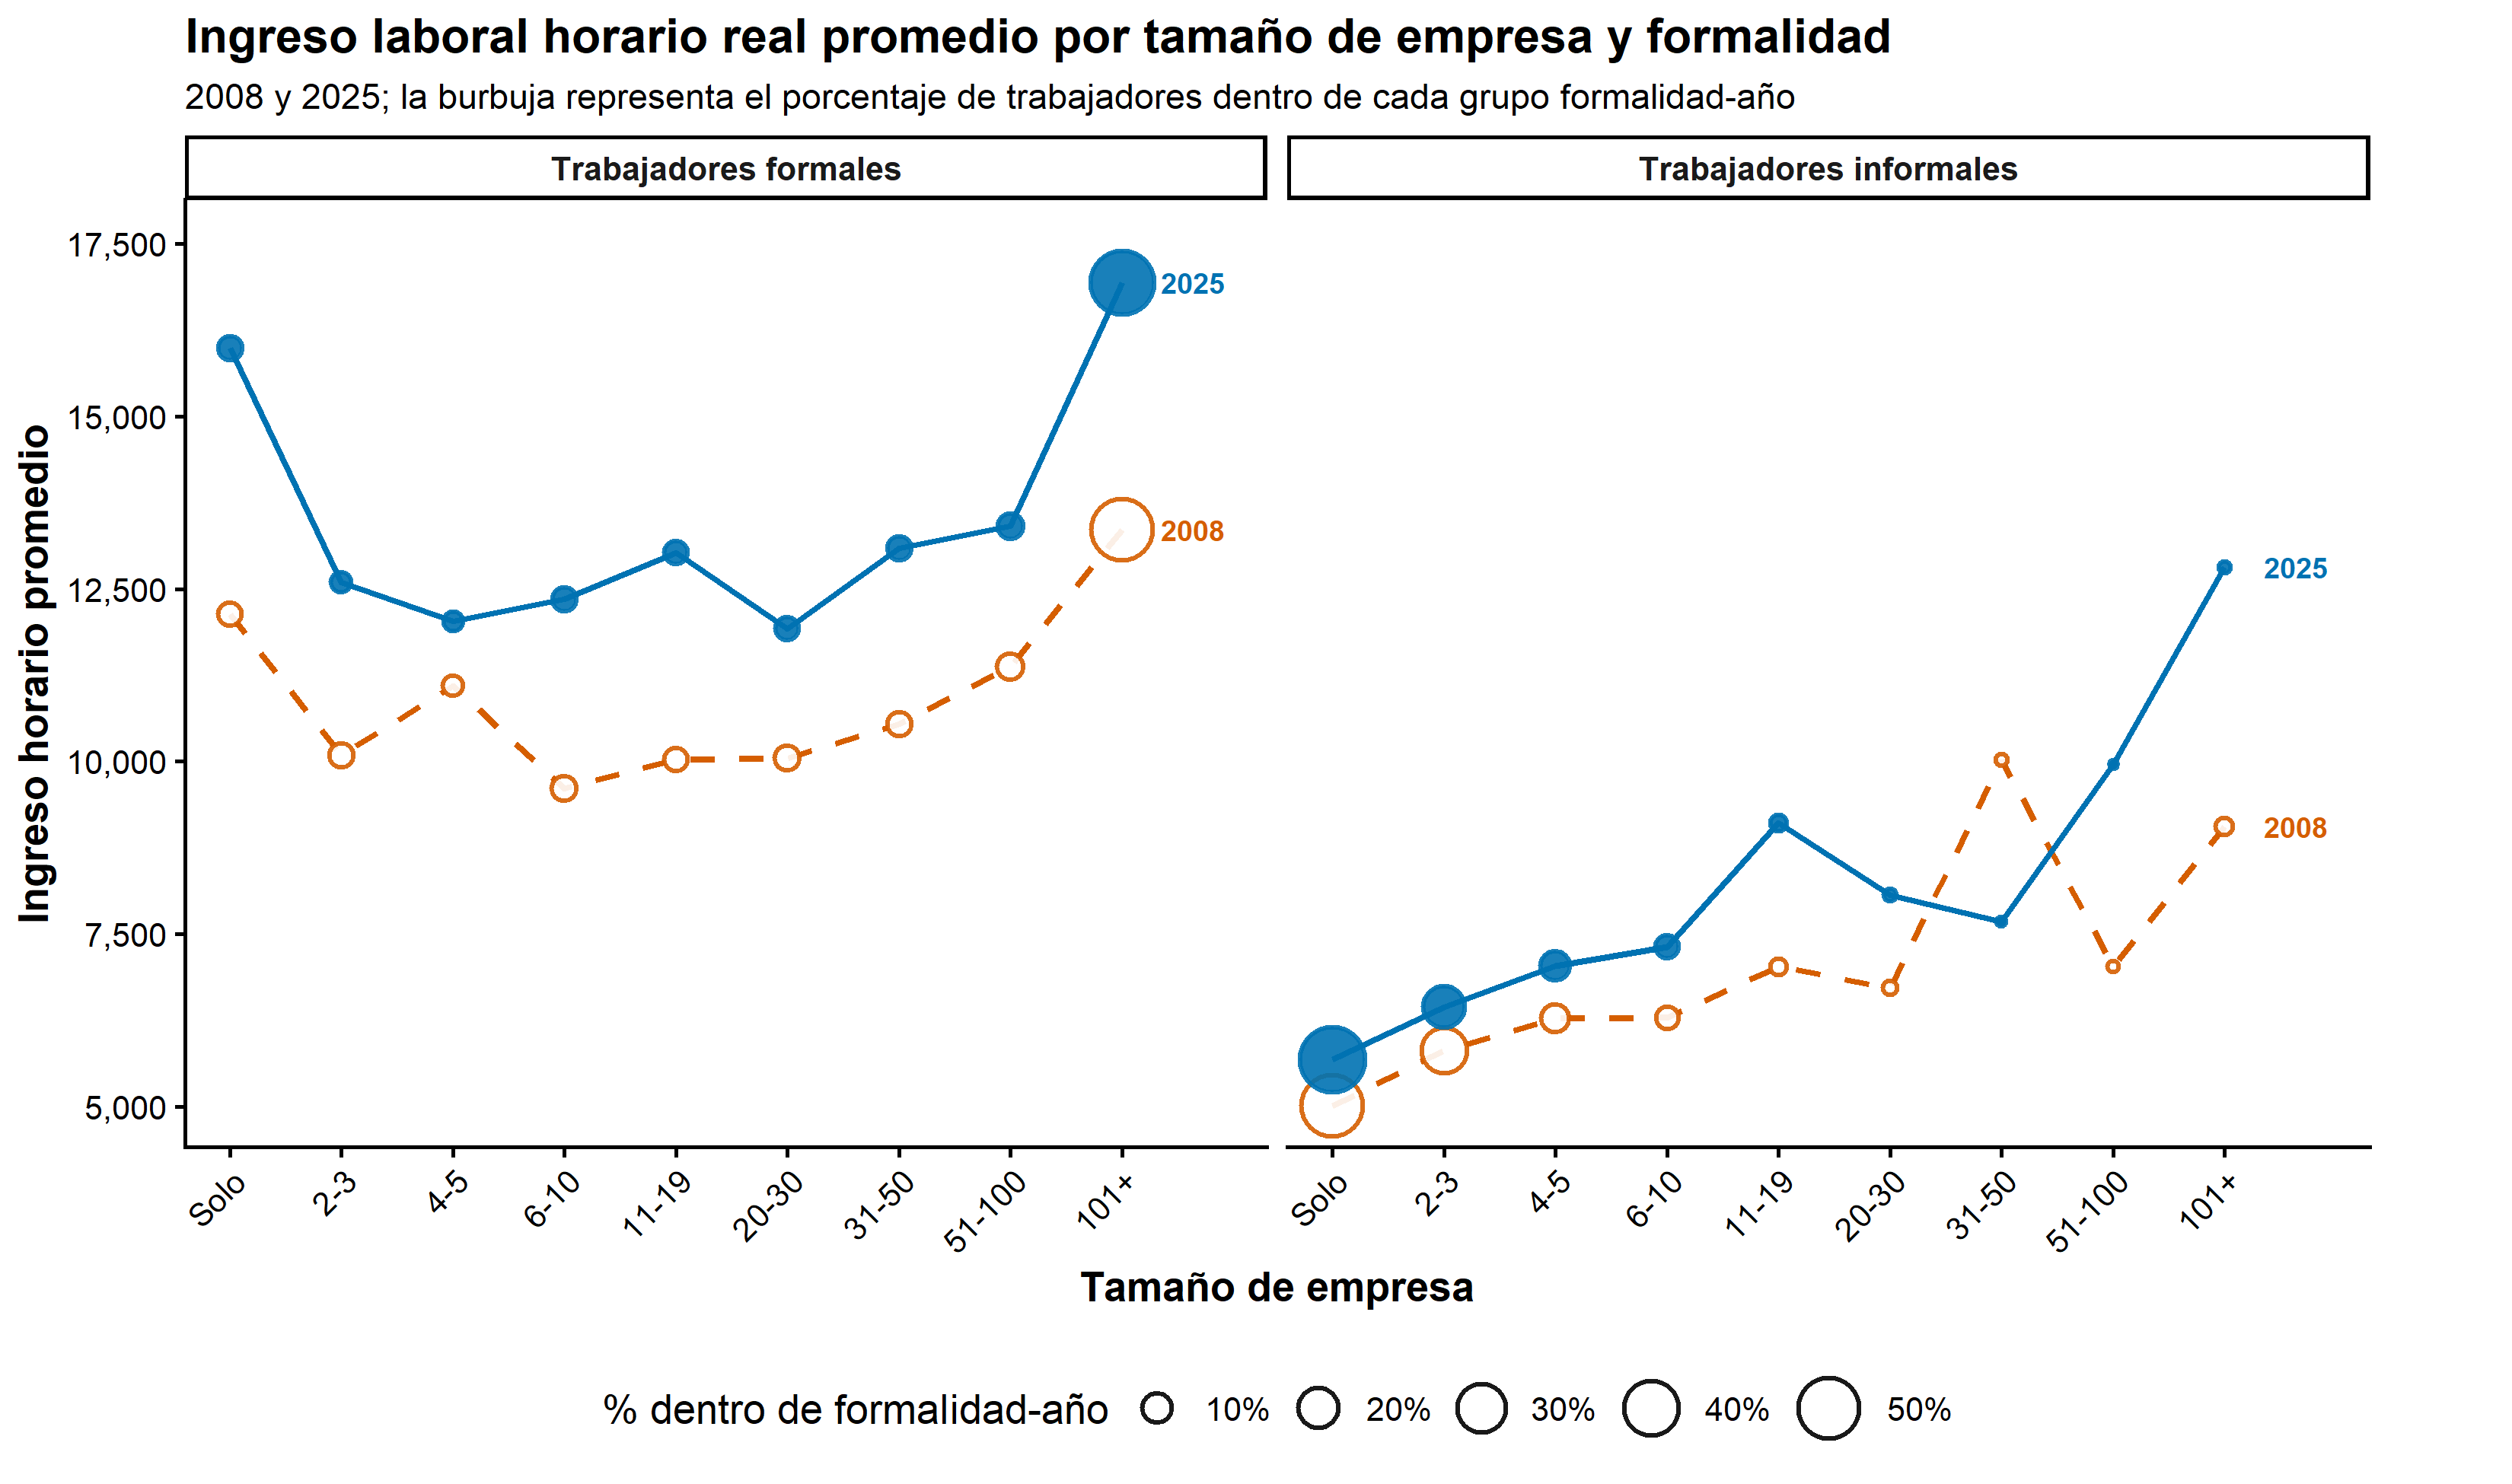
\includegraphics[width=0.94\textwidth,height=0.79\textheight,keepaspectratio]{fig69_es.png}

  \fuente{La burbuja representa la participación dentro de cada grupo formalidad-año.}
\end{frame}

\begin{frame}{Cómo leer la U de los formales}
  \idea{La U entre trabajadores formales no debe leerse como si todos los formales solos fueran profesionales de altos ingresos.}

  \vspace{0.35cm}
  \begin{itemize}
    \item El trabajo formal solo es una categoría seleccionada y heterogénea.
    \item En 2025, 82,1\% de los formales solos eran trabajadores por cuenta propia.
    \item 50,9\% tenía educación superior.
    \item Pero también había concentración en servicio doméstico y transporte.
    \item Por eso la U descriptiva puede reflejar composición del grupo de formales solos, no una prima pura del trabajo solo formal.
  \end{itemize}
\end{frame}

\begin{frame}{La prima bruta aparece dentro de hombres y mujeres}
  \centering
  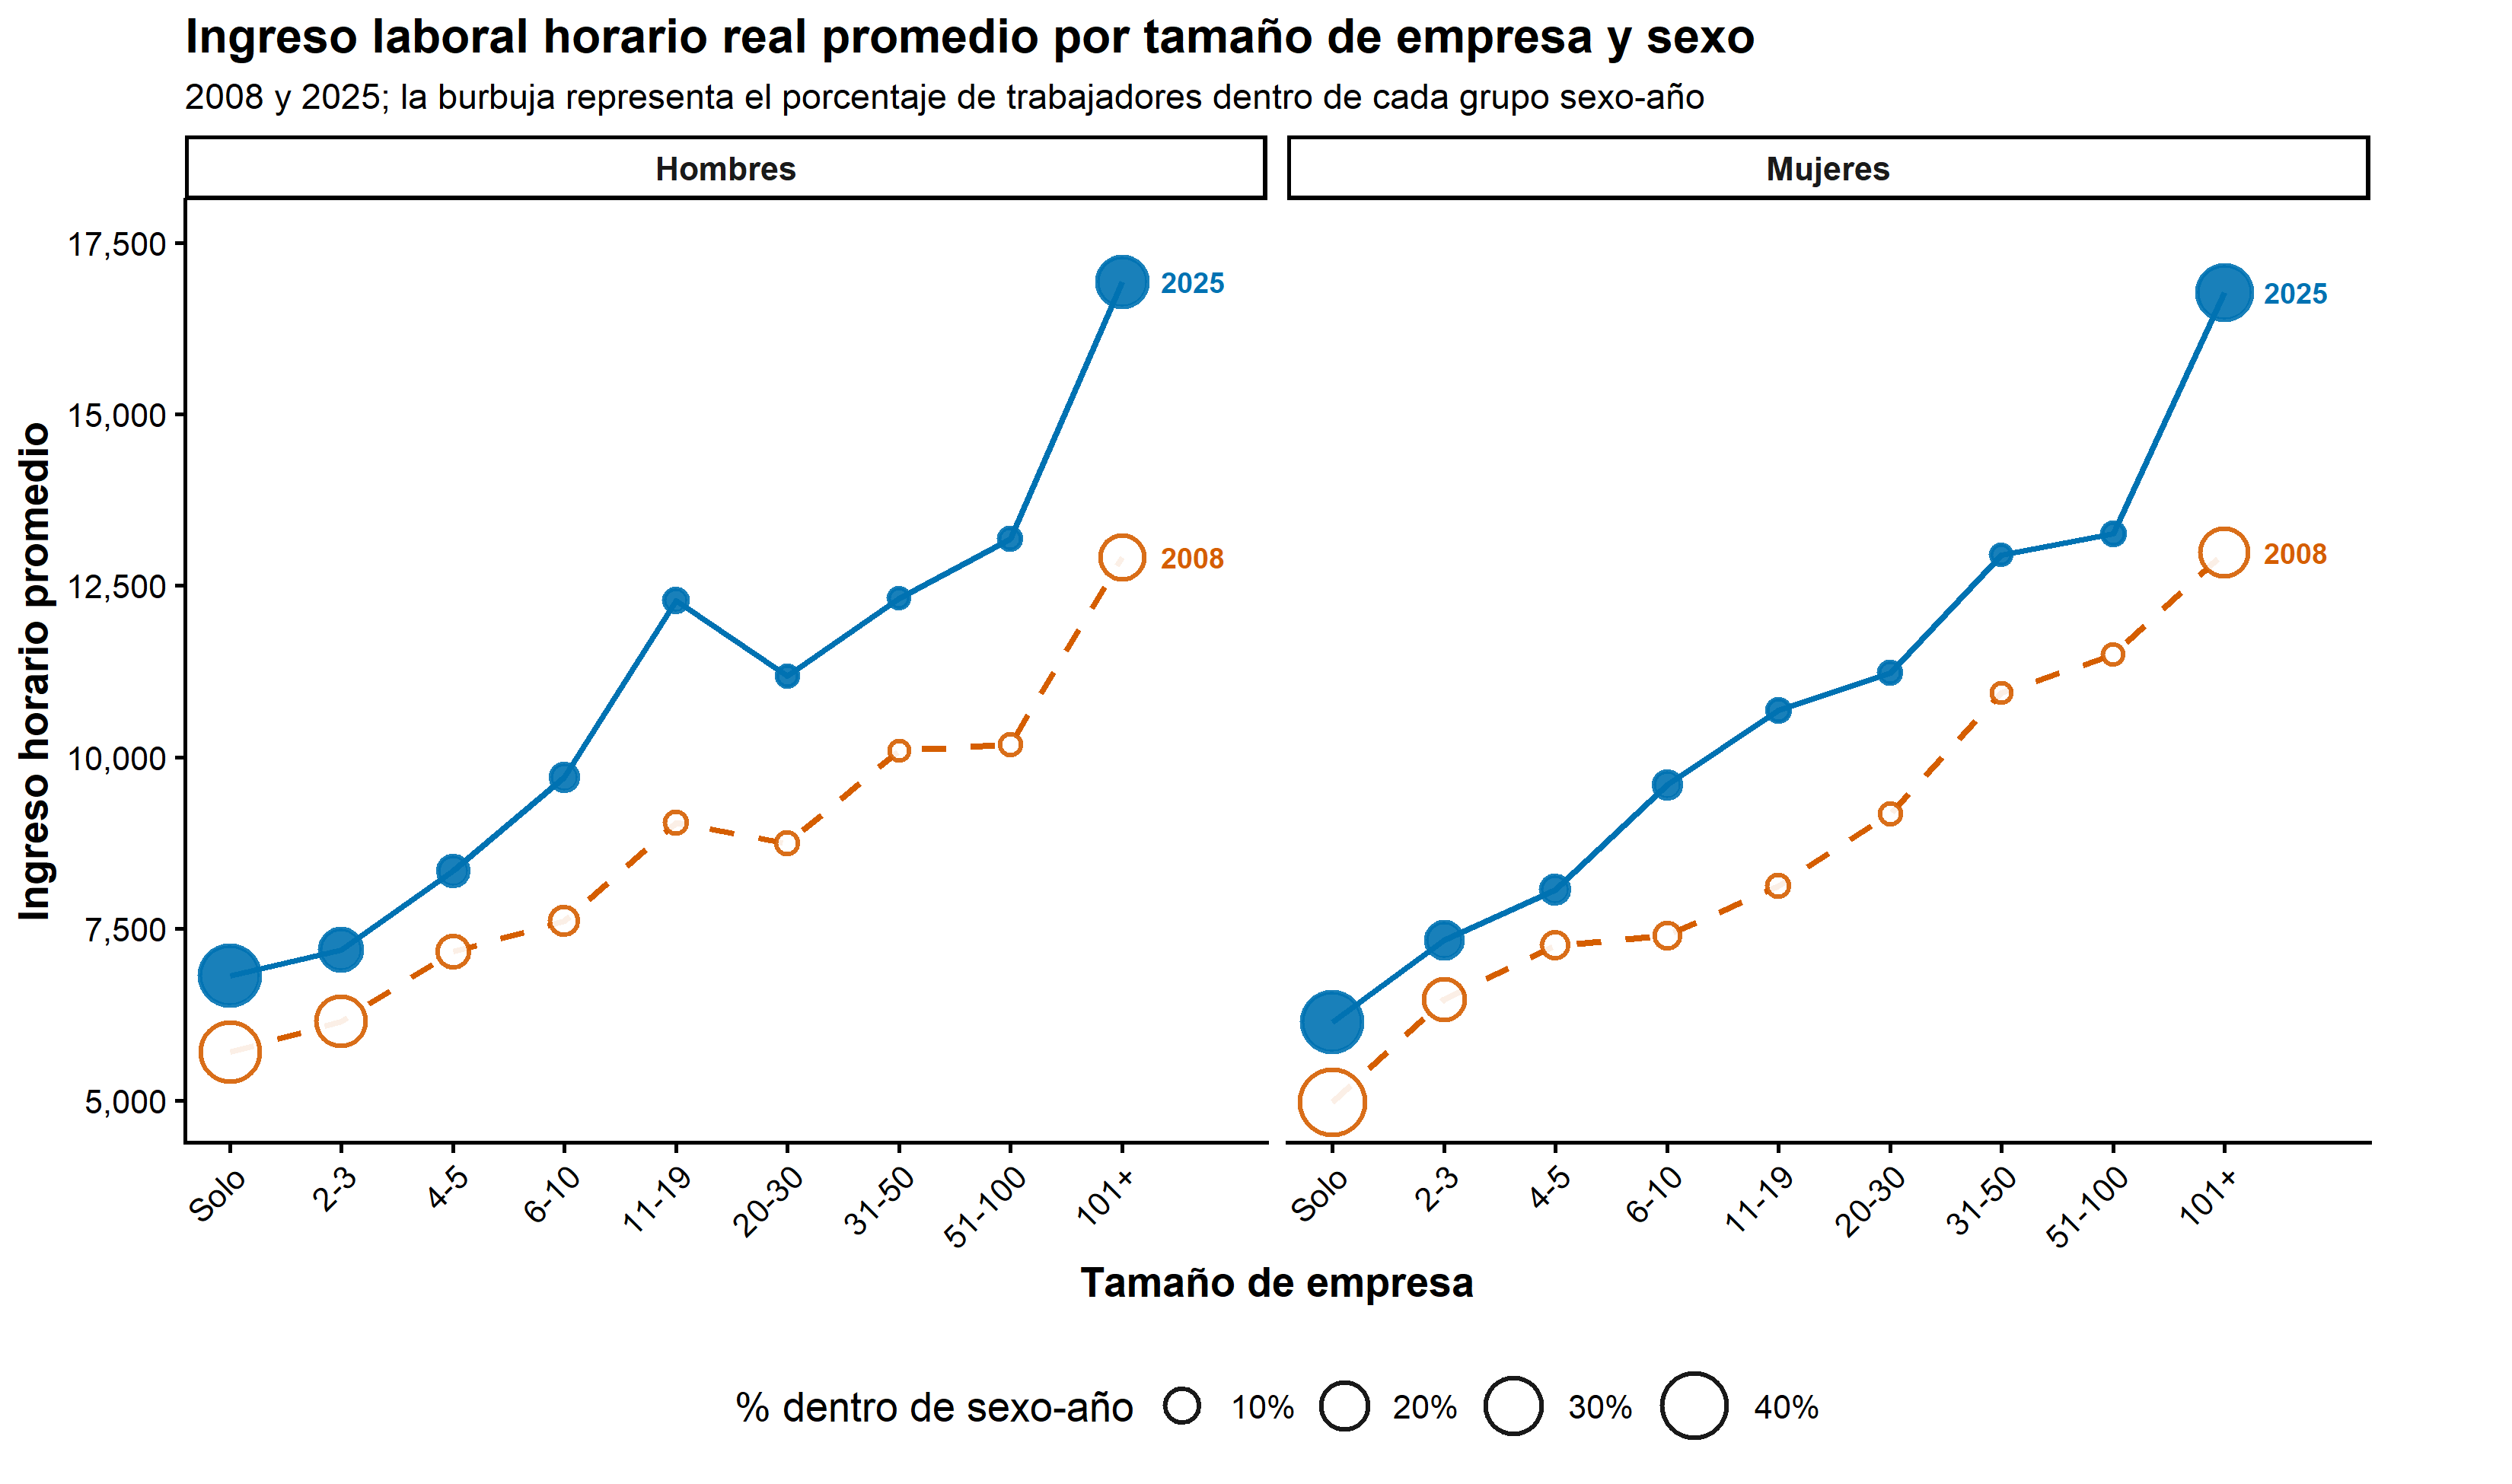
\includegraphics[width=0.94\textwidth,height=0.79\textheight,keepaspectratio]{fig70_es.png}

  \fuente{La brecha por sexo dentro de cada tamaño es pequeña frente a la brecha entre trabajo solo y firmas grandes.}
\end{frame}

\begin{frame}{La prima bruta aparece dentro de cada nivel educativo}
  \centering
  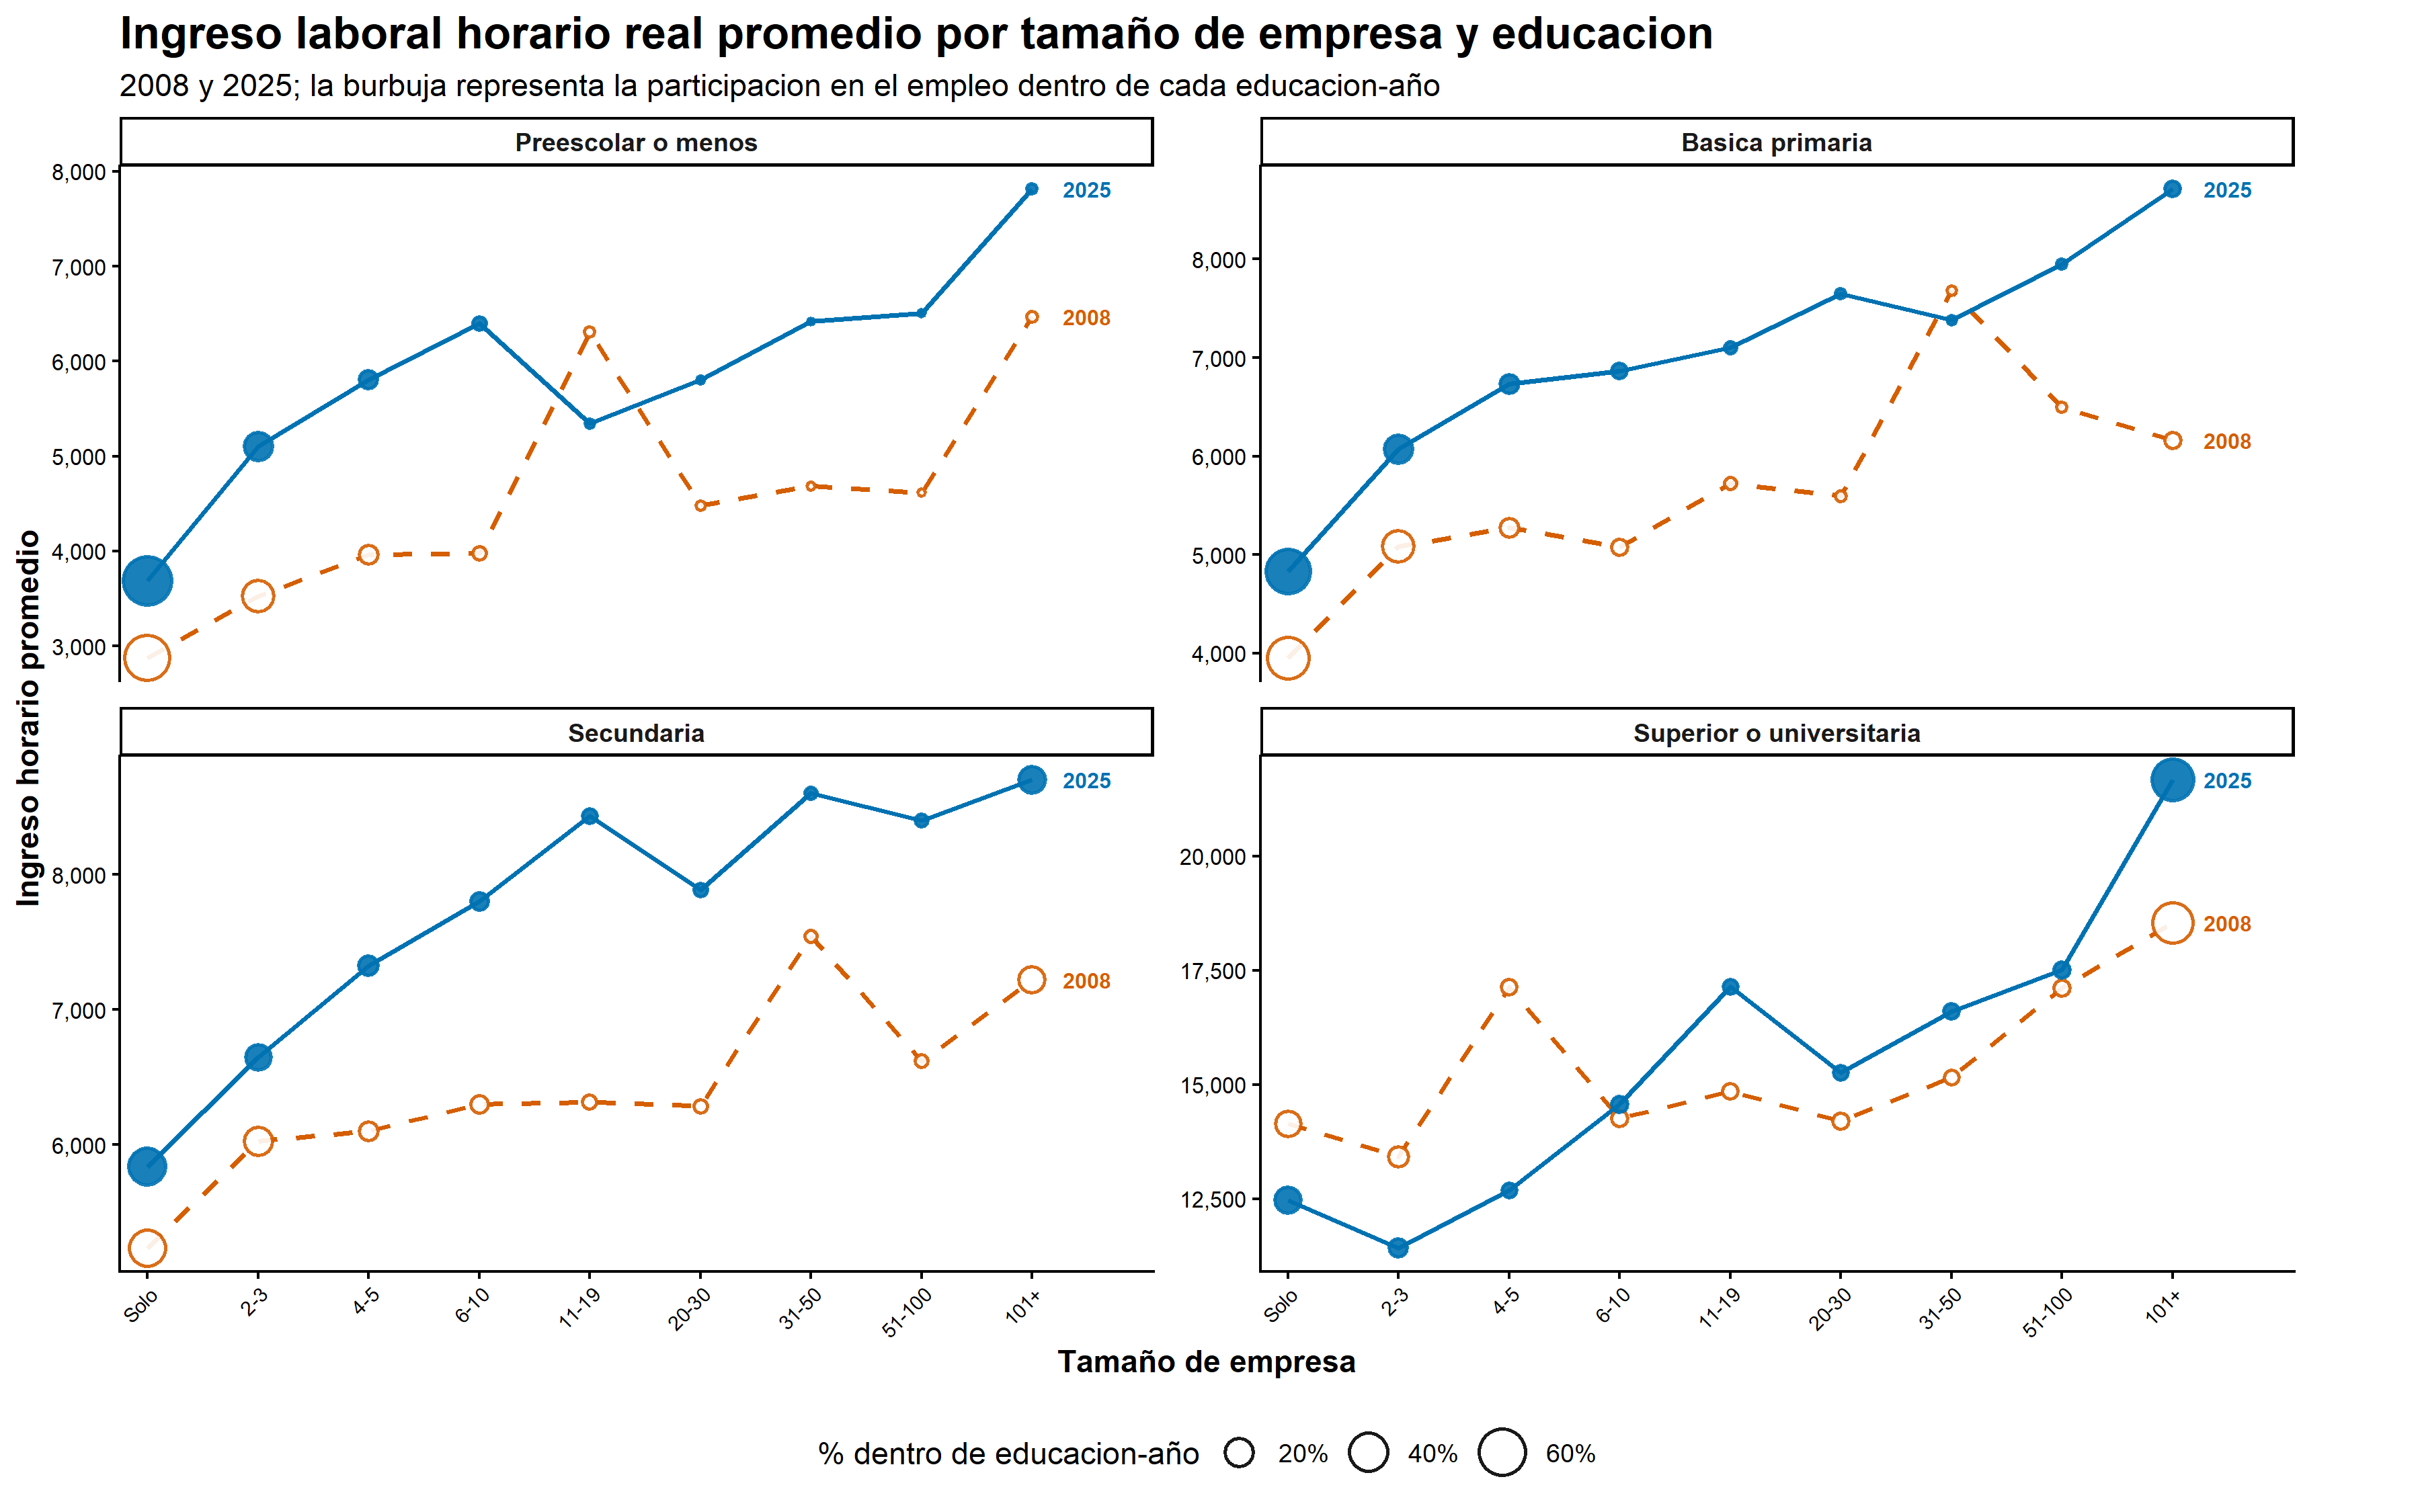
\includegraphics[width=0.96\textwidth,height=0.79\textheight,keepaspectratio]{fig72_es.png}

  \fuente{La prima 101+/solo fue 2,1 para preescolar o menos, 1,8 para primaria, 1,5 para secundaria y 1,7 para educación superior.}
\end{frame}

\begin{frame}{La prima también aparece en la mayoría de sectores}
  \centering
  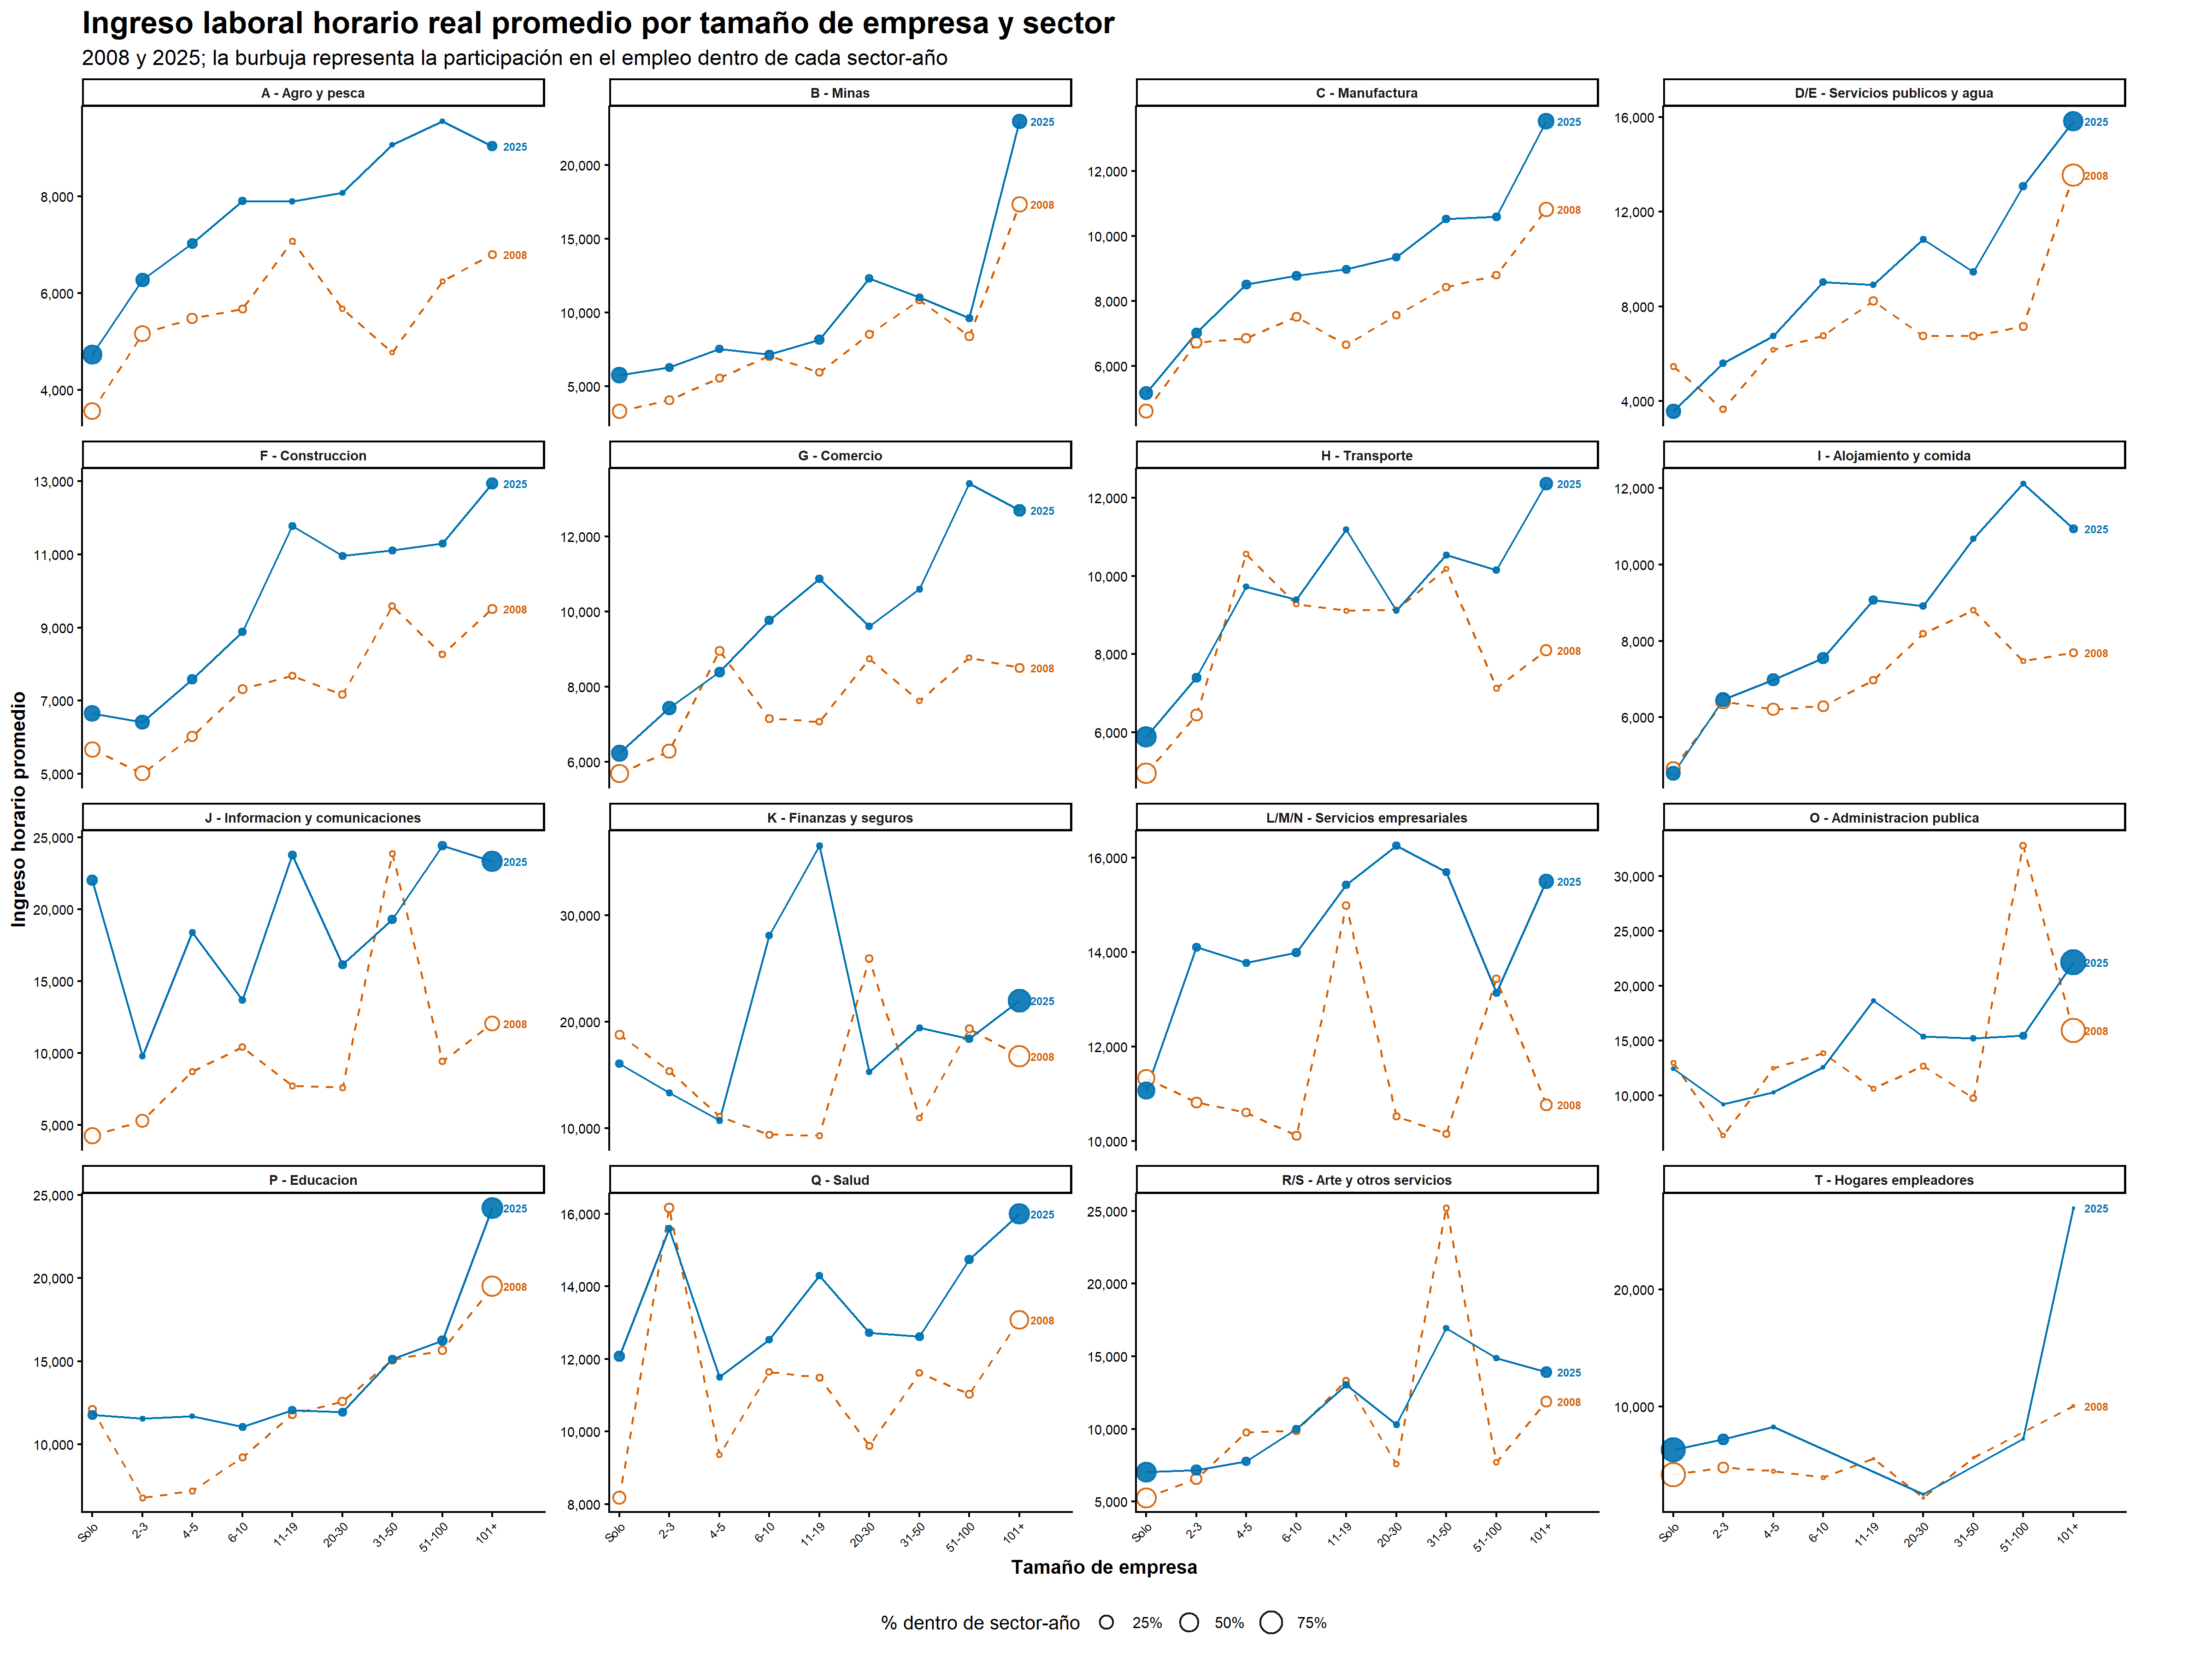
\includegraphics[width=0.98\textwidth,height=0.80\textheight,keepaspectratio]{fig71_es.png}

  \fuente{En 2025, la remuneración en 101+ superó la de trabajo solo en los 16 sectores incluidos.}
\end{frame}

\sectionframe{3. Prima condicional por tamaño de empresa}

\begin{frame}{Especificación principal}
  \idea{Estimamos brechas salariales condicionales, no efectos causales.}

  \vspace{0.2cm}
  \[
    \ln(w_{ist}) =
    \alpha
    + \sum_{g \neq Solo} \beta_g \mathbf{1}\{Size_{ist}=g\}
    + X_{ist}'\gamma
    + \lambda_{s \times t}
    + \varepsilon_{ist}
  \]

  \vspace{0.25cm}
  \begin{itemize}
    \item \(w_{ist}\): ingreso laboral real por hora.
    \item \(X_{ist}\): sexo, edad, edad al cuadrado, educación y formalidad.
    \item \(\lambda_{s \times t}\): efectos fijos sector-año.
    \item Los coeficientes se transforman como \(100 \times [\exp(\hat{\beta}_g)-1]\).
  \end{itemize}
\end{frame}

\begin{frame}{Qué pasa cuando agregamos controles}
  \idea{La prima de las firmas 101+ cae mucho, pero no desaparece.}

  \vspace{0.25cm}
  \begin{center}
  \scriptsize
  \setlength{\tabcolsep}{3pt}
  \begin{tabular}{p{0.34\textwidth}cp{0.38\textwidth}}
    \toprule
    Especificación & Coeficiente 101+ & Interpretación \\
    \midrule
    Sin controles & 1,019 & Brecha bruta muy grande \\
    + efectos fijos sector-año & 0,819 & Parte responde al sector y al año \\
    + sexo, edad y educación & 0,598 & Parte responde a composición del trabajador \\
    + formalidad & 0,359 & Prima condicional de 43,2\% \\
    \bottomrule
  \end{tabular}
  \end{center}

  \vspace{0.35cm}
  \begin{center}
  \begin{minipage}{0.88\textwidth}
  \scriptsize
  Aproximadamente dos terceras partes de la brecha bruta 101+ se absorben al agregar controles observables.
  \end{minipage}
  \end{center}
\end{frame}

\begin{frame}{Prima condicional por tamaño}
  \centering
  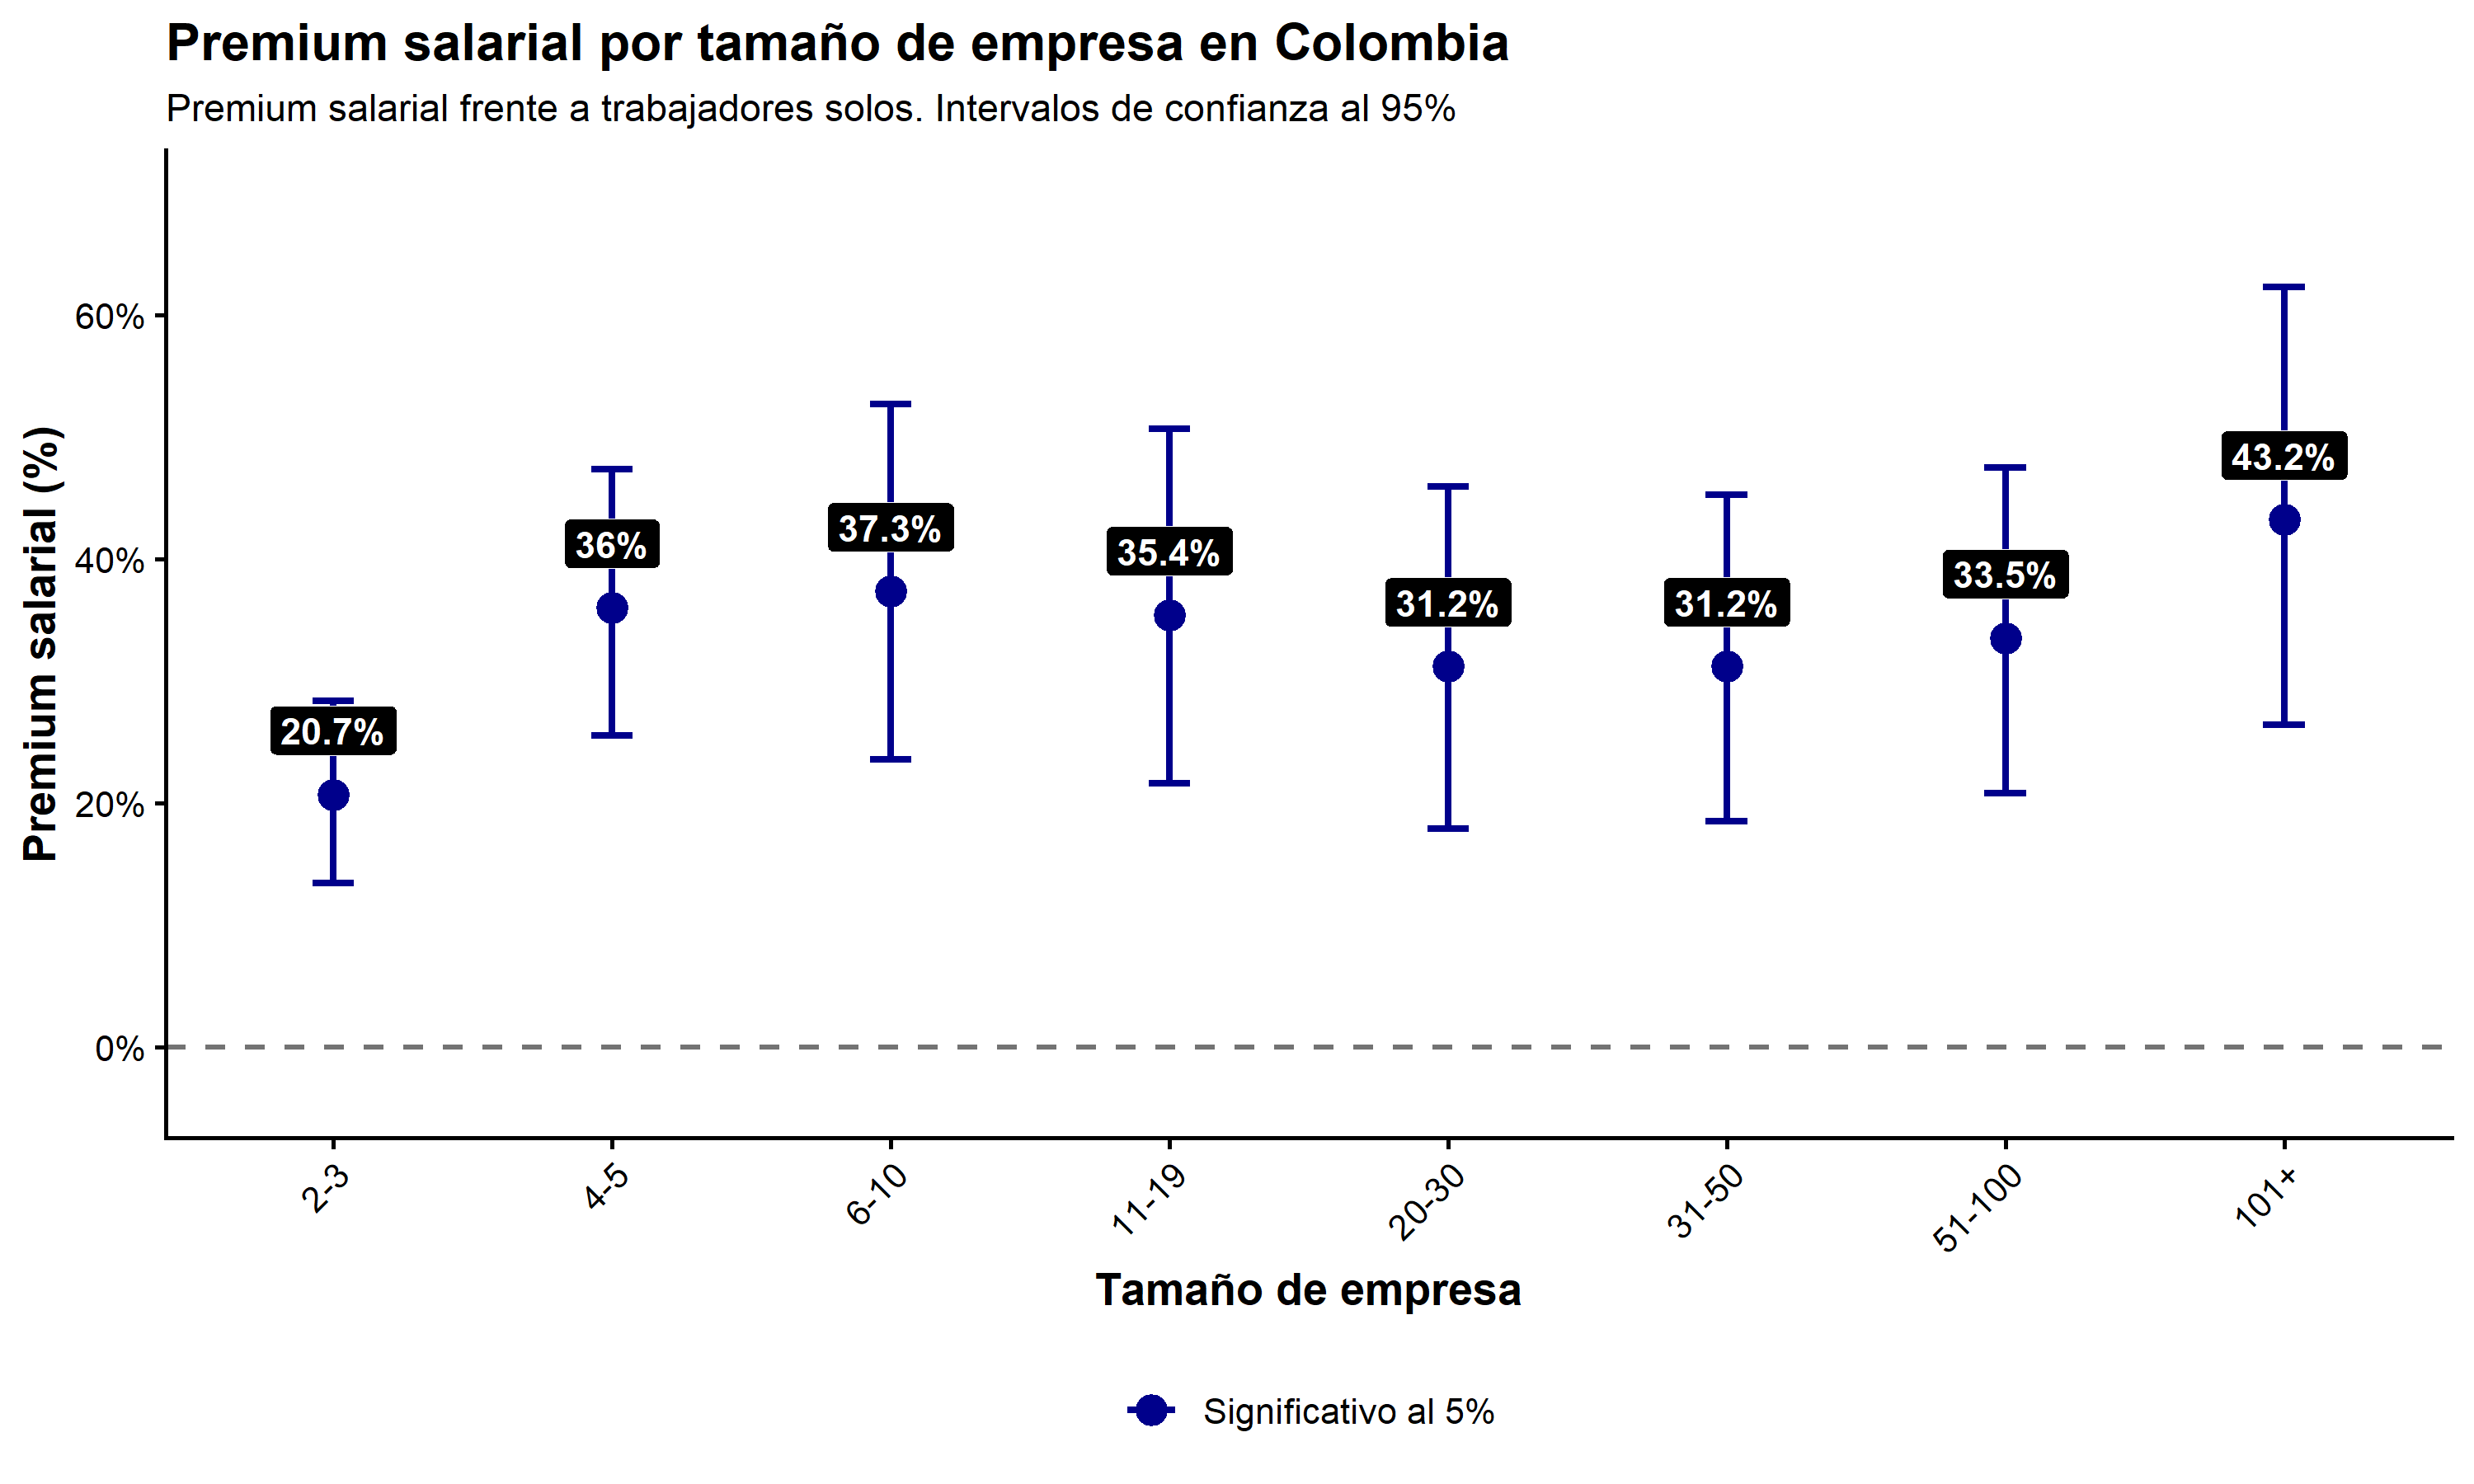
\includegraphics[width=0.92\textwidth,height=0.80\textheight,keepaspectratio]{fig57_es.png}

  \fuente{Prima relativa a trabajadores solos, después de controles por sexo, edad, educación, formalidad y efectos fijos sector-año.}
\end{frame}

\begin{frame}{Resultado principal}
  \begin{columns}[T,totalwidth=\textwidth]
    \begin{column}{0.38\textwidth}
      \bigstat{43,2\%}{prima condicional en firmas de 101+ frente a trabajadores solos}{cjcblue}
    \end{column}
    \begin{column}{0.58\textwidth}
      \vspace{0.25cm}
      \begin{itemize}
        \item La prima condicional es positiva en todas las categorías de tamaño.
        \item Los intervalos de confianza excluyen cero en la especificación principal.
        \item El resultado no se explica solo por la diferencia formal-informal.
        \item Tampoco debe interpretarse como un experimento donde el mismo trabajador cambia de firma.
      \end{itemize}
    \end{column}
  \end{columns}
\end{frame}

\sectionframe{4. Evolución en el tiempo}

\begin{frame}{Qué significa que la prima se empine o se aplane}
  \idea{La evolución de la prima mide si el tamaño de empresa se volvió más o menos asociado con la remuneración.}

  \vspace{0.35cm}
  \begin{itemize}
    \item Una prima más empinada significa que las diferencias salariales por tamaño aumentaron.
    \item Una prima más plana significa que las diferencias salariales por tamaño se redujeron.
    \item La prueba no identifica por sí sola si el cambio viene de salarios más altos abajo, salarios más bajos arriba o cambios de composición.
  \end{itemize}
\end{frame}

\begin{frame}{Prima condicional a través del tiempo}
  \centering
  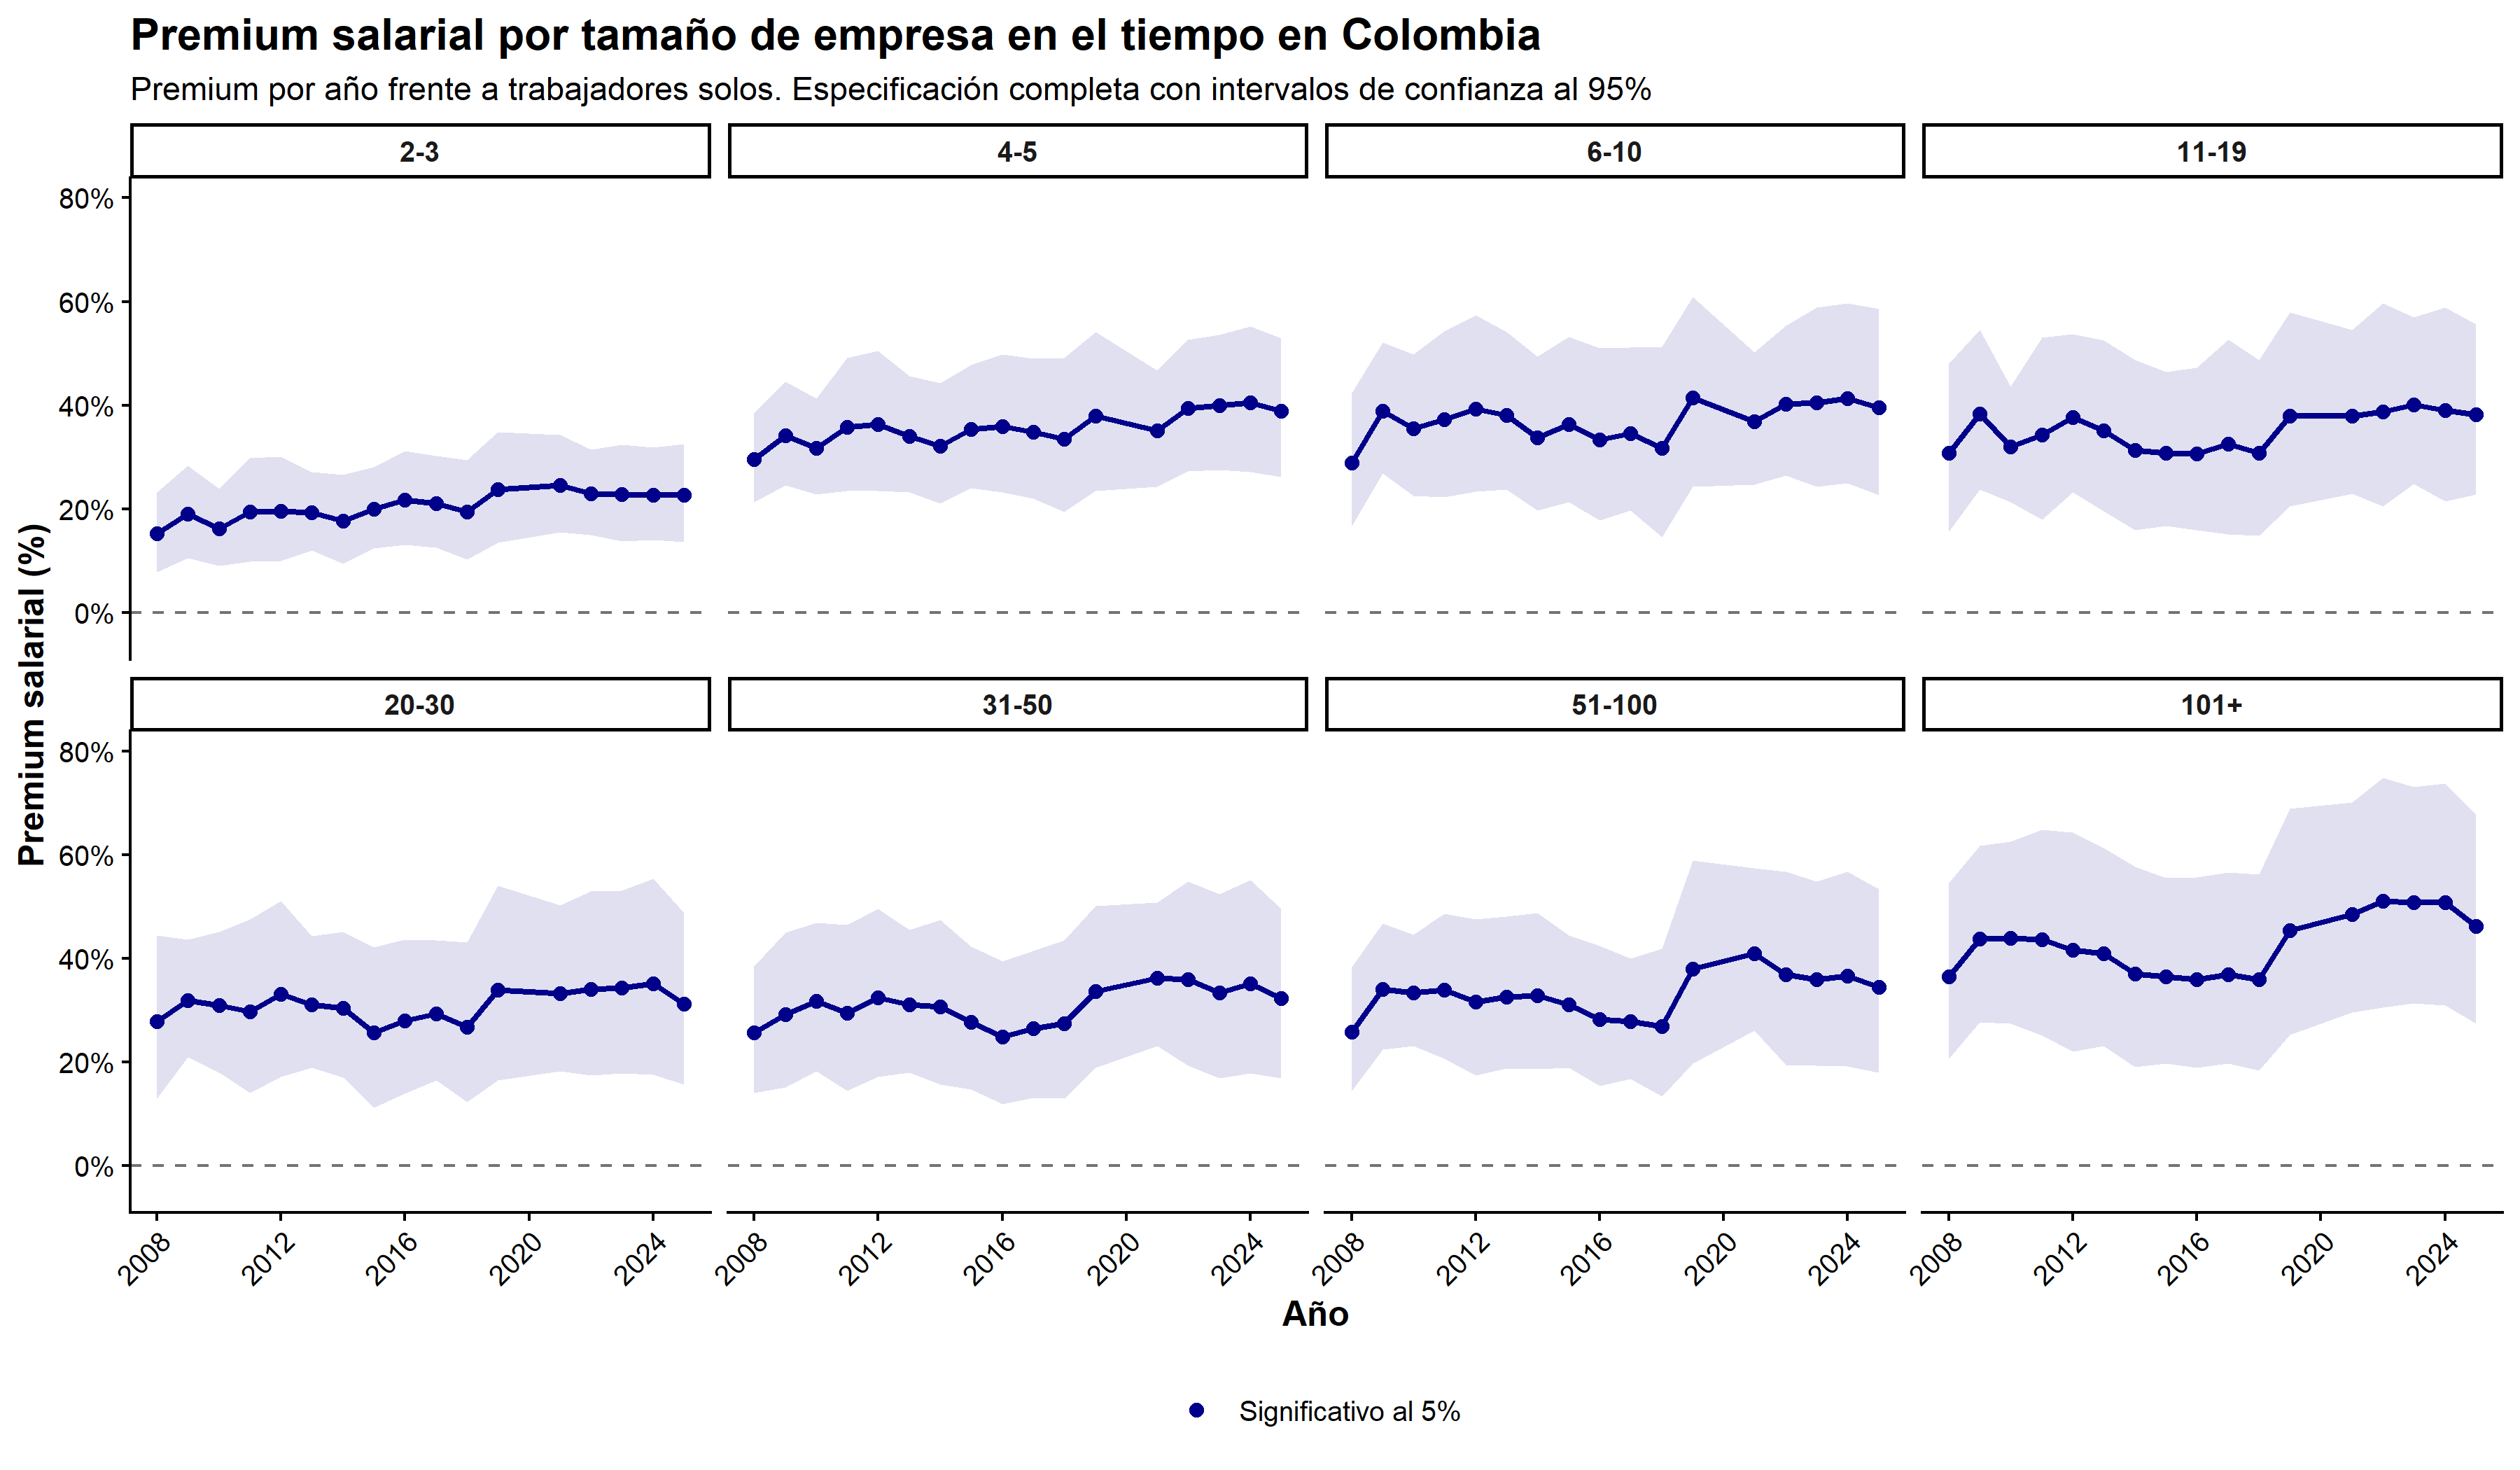
\includegraphics[width=0.96\textwidth,height=0.80\textheight,keepaspectratio]{fig59_es.png}

  \fuente{Estimaciones anuales de la especificación principal. Se omite 2020.}
\end{frame}

\begin{frame}{La evidencia sugiere persistencia, no una tendencia clara}
  \idea{Los puntos estimados sugieren aumento, pero las pruebas no permiten afirmar que la prima se haya empinado de manera sistemática.}

  \vspace{0.3cm}
  \begin{center}
  \small
  \begin{tabular}{lcc}
    \toprule
    Tamaño & Cambio implícito 2008--2025 & Lectura \\
    \midrule
    20--30 & 3,2\% & No significativo al 5\% \\
    51--100 & 6,7\% & No significativo al 5\% \\
    101+ & 7,9\% & No significativo al 5\% \\
    \bottomrule
  \end{tabular}
  \end{center}

  \vspace{0.35cm}
  {\small Colombia no se ve como un caso de convergencia clara ni de divergencia estadísticamente concluyente. El resultado más defendible es persistencia.}
\end{frame}

\sectionframe{5. Formalidad y no linealidades}

\begin{frame}{Por qué separar formales e informales}
  \idea{La formalidad puede mediar y modificar la prima por tamaño.}

  \vspace{0.35cm}
  \begin{itemize}
    \item Puede mediarla porque las firmas grandes tienen más probabilidad de ofrecer empleos formales.
    \item Puede modificarla porque la relación entre tamaño y salarios puede ser distinta dentro del empleo formal e informal.
    \item Si el tamaño importa sobre todo dentro del empleo informal, la discusión de política cambia.
  \end{itemize}
\end{frame}

\begin{frame}{Especificación con interacción por formalidad}
  \[
    \ln(w_{ist}) =
    \alpha + \phi Formal_{ist}
    + \sum_{g \neq Solo}(\beta_g + \theta_g Formal_{ist})
      \mathbf{1}\{Size_{ist}=g\}
    + X_{ist}'\gamma
    + \lambda_{s \times t}
    + \varepsilon_{ist}
  \]

  \vspace{0.25cm}
  \begin{itemize}
    \item \(\beta_g\): prima por tamaño entre informales.
    \item \(\beta_g+\theta_g\): prima por tamaño entre formales.
    \item \(\phi+\theta_g\): brecha formal-informal dentro del tamaño \(g\).
  \end{itemize}
\end{frame}

\begin{frame}{La prima condicional es mucho más fuerte entre informales}
  \centering
  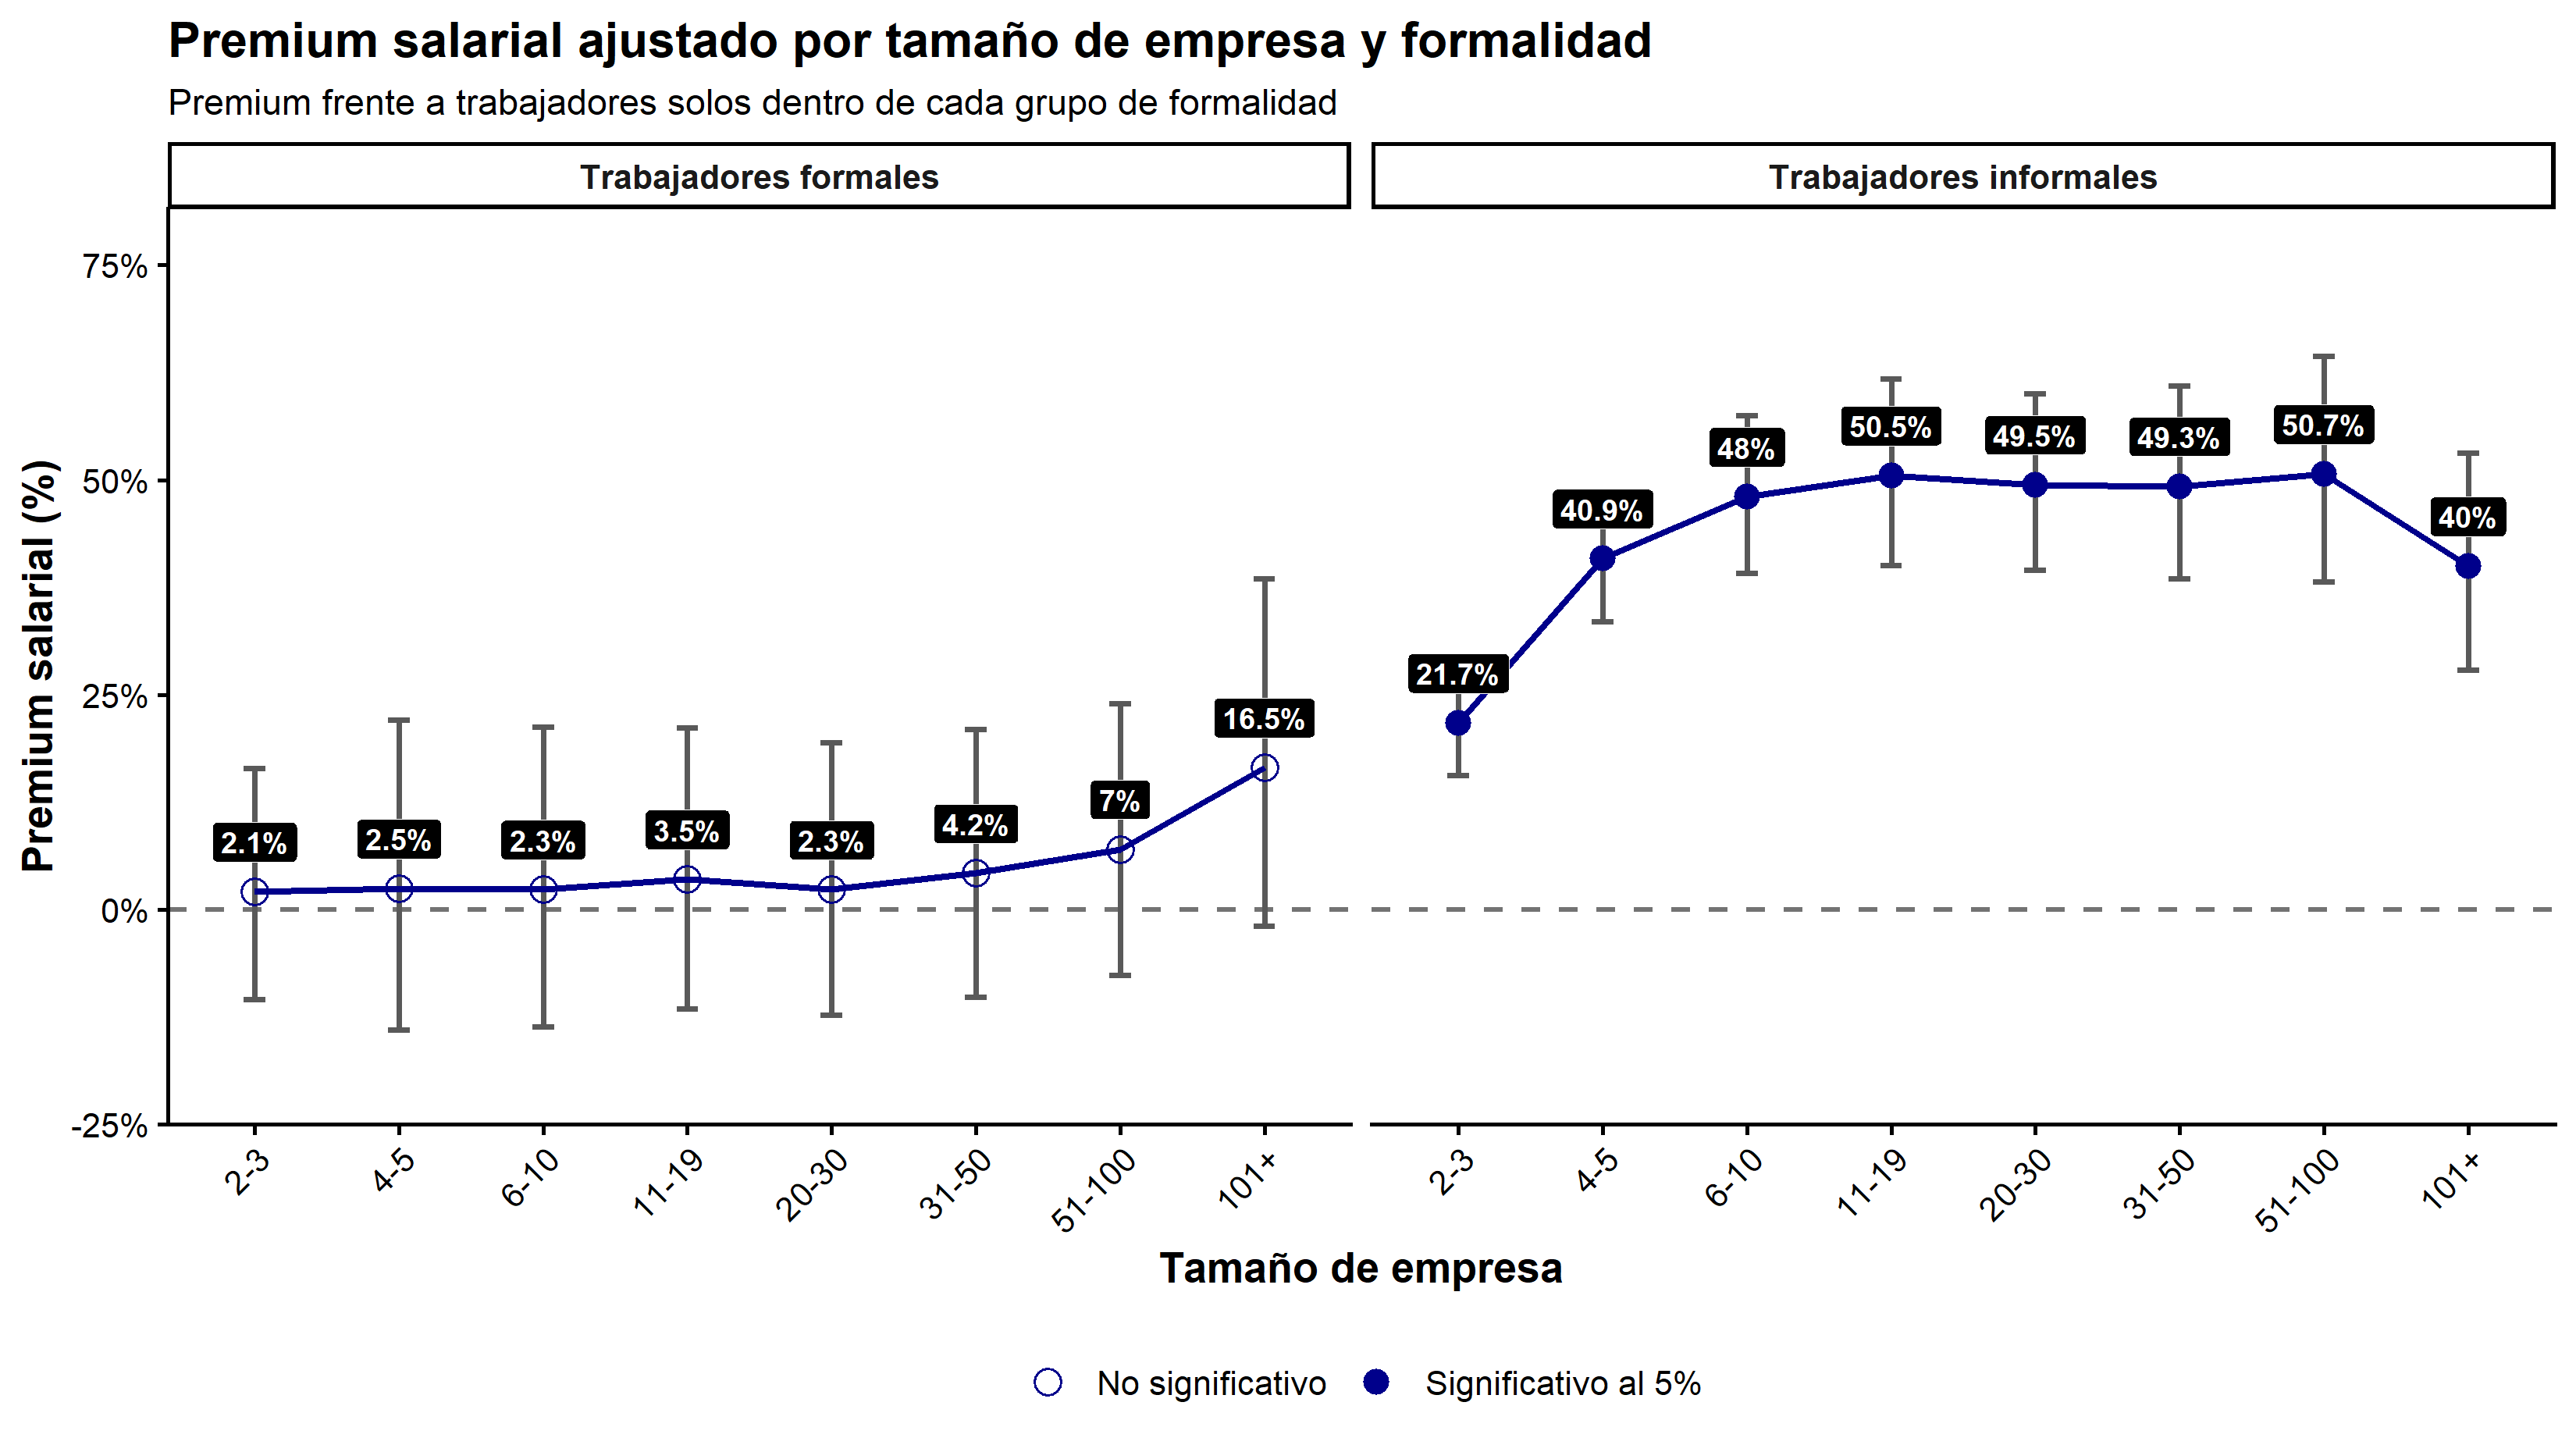
\includegraphics[width=0.94\textwidth,height=0.80\textheight,keepaspectratio]{fig74_es.png}

  \fuente{Prima relativa a trabajadores solos dentro del mismo grupo de formalidad.}
\end{frame}

\begin{frame}{Lectura de la figura por formalidad}
  \begin{columns}[T,totalwidth=\textwidth]
    \begin{column}{0.48\textwidth}
      \idea{Informales}
      \vspace{0.25cm}
      \begin{itemize}
        \item La prima es positiva y significativa en todas las categorías.
        \item En 6--100 trabajadores está alrededor de 48--51\%.
        \item En 101+ sigue siendo alta: 40,0\%.
      \end{itemize}
    \end{column}
    \begin{column}{0.48\textwidth}
      \idea{Formales}
      \vspace{0.25cm}
      \begin{itemize}
        \item La prima frente a formales solos es pequeña y menos precisa.
        \item La estimación para 101+ es 16,5\%, pero no significativa al 5\%.
        \item La comparación relevante dentro del formal también puede ser 101+ frente a firmas formales intermedias.
      \end{itemize}
    \end{column}
  \end{columns}
\end{frame}

\begin{frame}{Dentro del empleo formal sí hay una comparación relevante}
  \idea{Los trabajadores formales en firmas 101+ ganan más que trabajadores formales en firmas intermedias.}

  \vspace{0.25cm}
  \begin{center}
  \small
  \begin{tabular}{lcc}
    \toprule
    Comparación & Prima 101+ & Significancia \\
    \midrule
    101+ frente a formal solo & 16,5\% & No significativa al 5\% \\
    101+ frente a 2--3 & 14,2\% & Significativa \\
    101+ frente a 6--10 & 13,9\% & Significativa \\
    101+ frente a 20--30 & 13,9\% & Significativa \\
    101+ frente a 51--100 & 8,9\% & Significativa \\
    \bottomrule
  \end{tabular}
  \end{center}

  \vspace{0.25cm}
  {\small La conclusión no es que el tamaño no importe dentro del sector formal. La conclusión es que la prima formal es mucho menos general que la prima informal.}
\end{frame}

\begin{frame}{Formalidad aumenta el nivel salarial dentro de cada tamaño}
  \idea{La prima por tamaño es más fuerte entre informales, pero la formalidad sigue siendo central.}

  \vspace{0.25cm}
  \begin{center}
  \small
  \begin{tabular}{lcc}
    \toprule
    Tamaño & Prima formal-informal condicional & Lectura \\
    \midrule
    Solo & 68,8\% & Muy alta \\
    2--3 & 20,7\% & Positiva \\
    6--10 & 16,6\% & Positiva \\
    31--50 & 22,8\% & Positiva \\
    101+ & 40,6\% & Alta \\
    \bottomrule
  \end{tabular}
  \end{center}

  \vspace{0.25cm}
  {\small Los formales ganan más que los informales dentro de cada categoría de tamaño.}
\end{frame}

\begin{frame}{La diferencia por formalidad también se ve en 2008 y 2025}
  \centering
  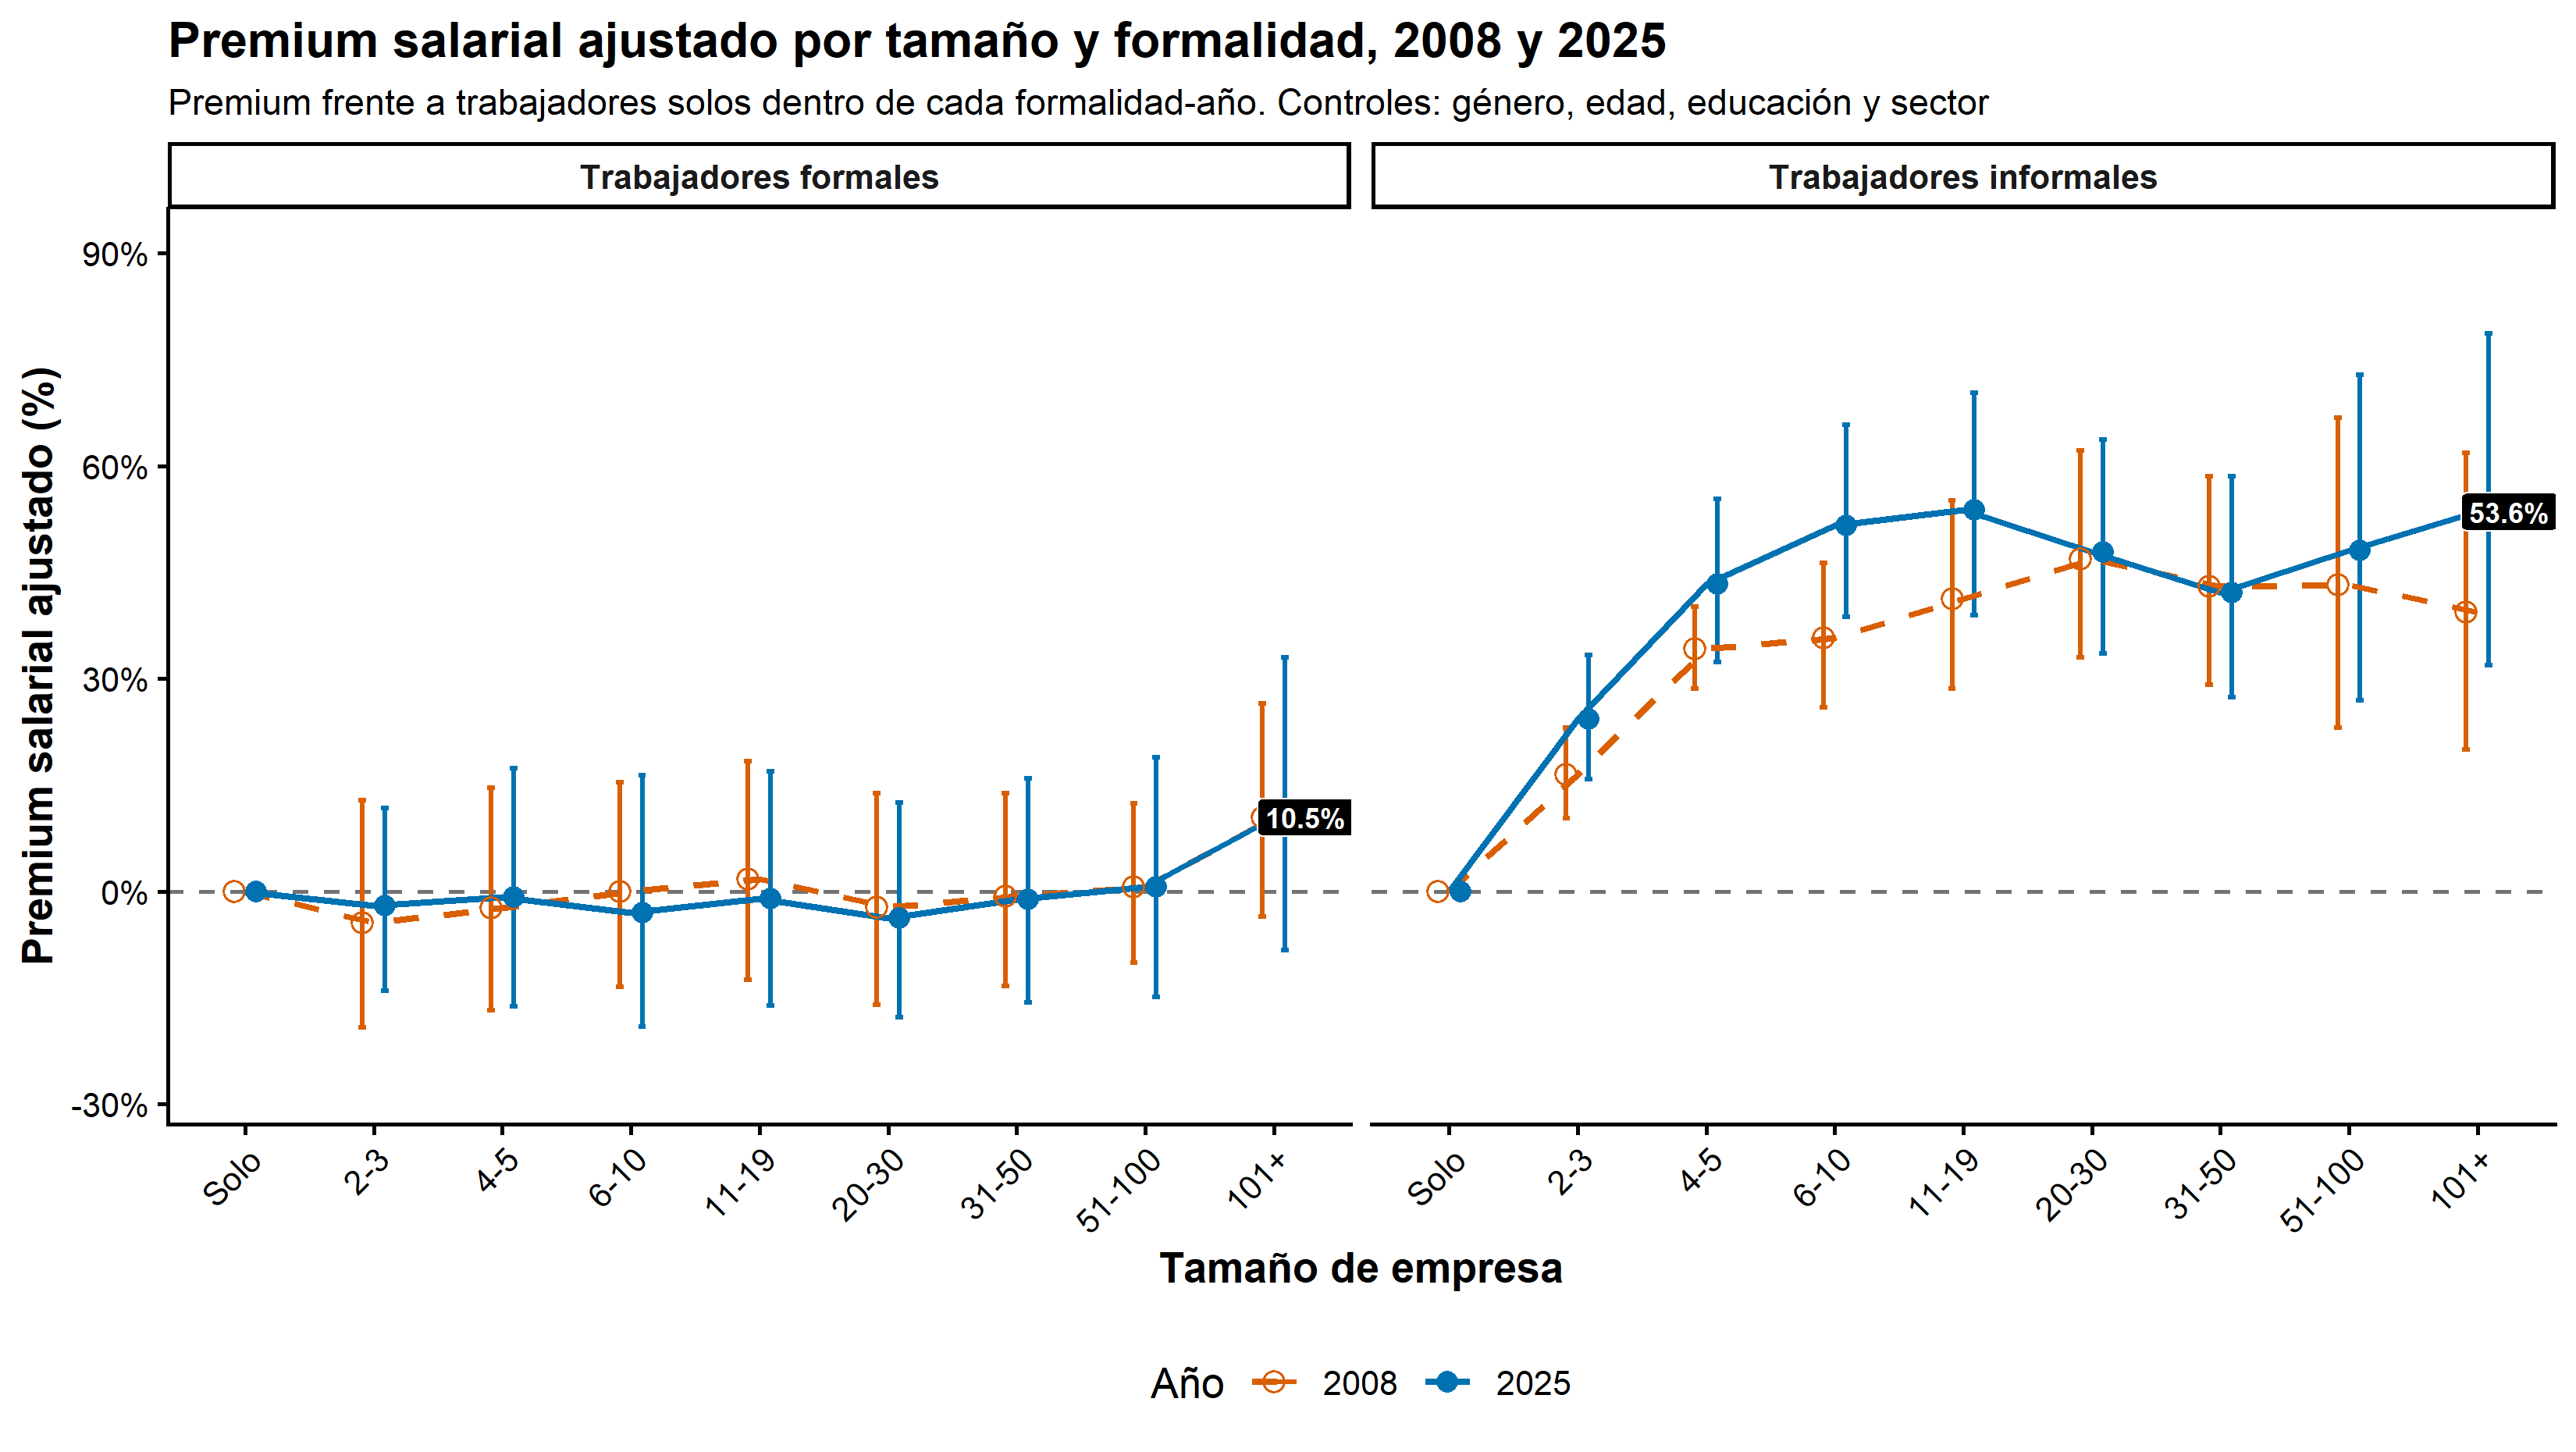
\includegraphics[width=0.95\textwidth,height=0.80\textheight,keepaspectratio]{fig76_es.png}

  \fuente{Estimaciones separadas para 2008 y 2025 con controles por sexo, edad, educación y sector.}
\end{frame}

\begin{frame}{La prima 101+ por formalidad a través del tiempo}
  \centering
  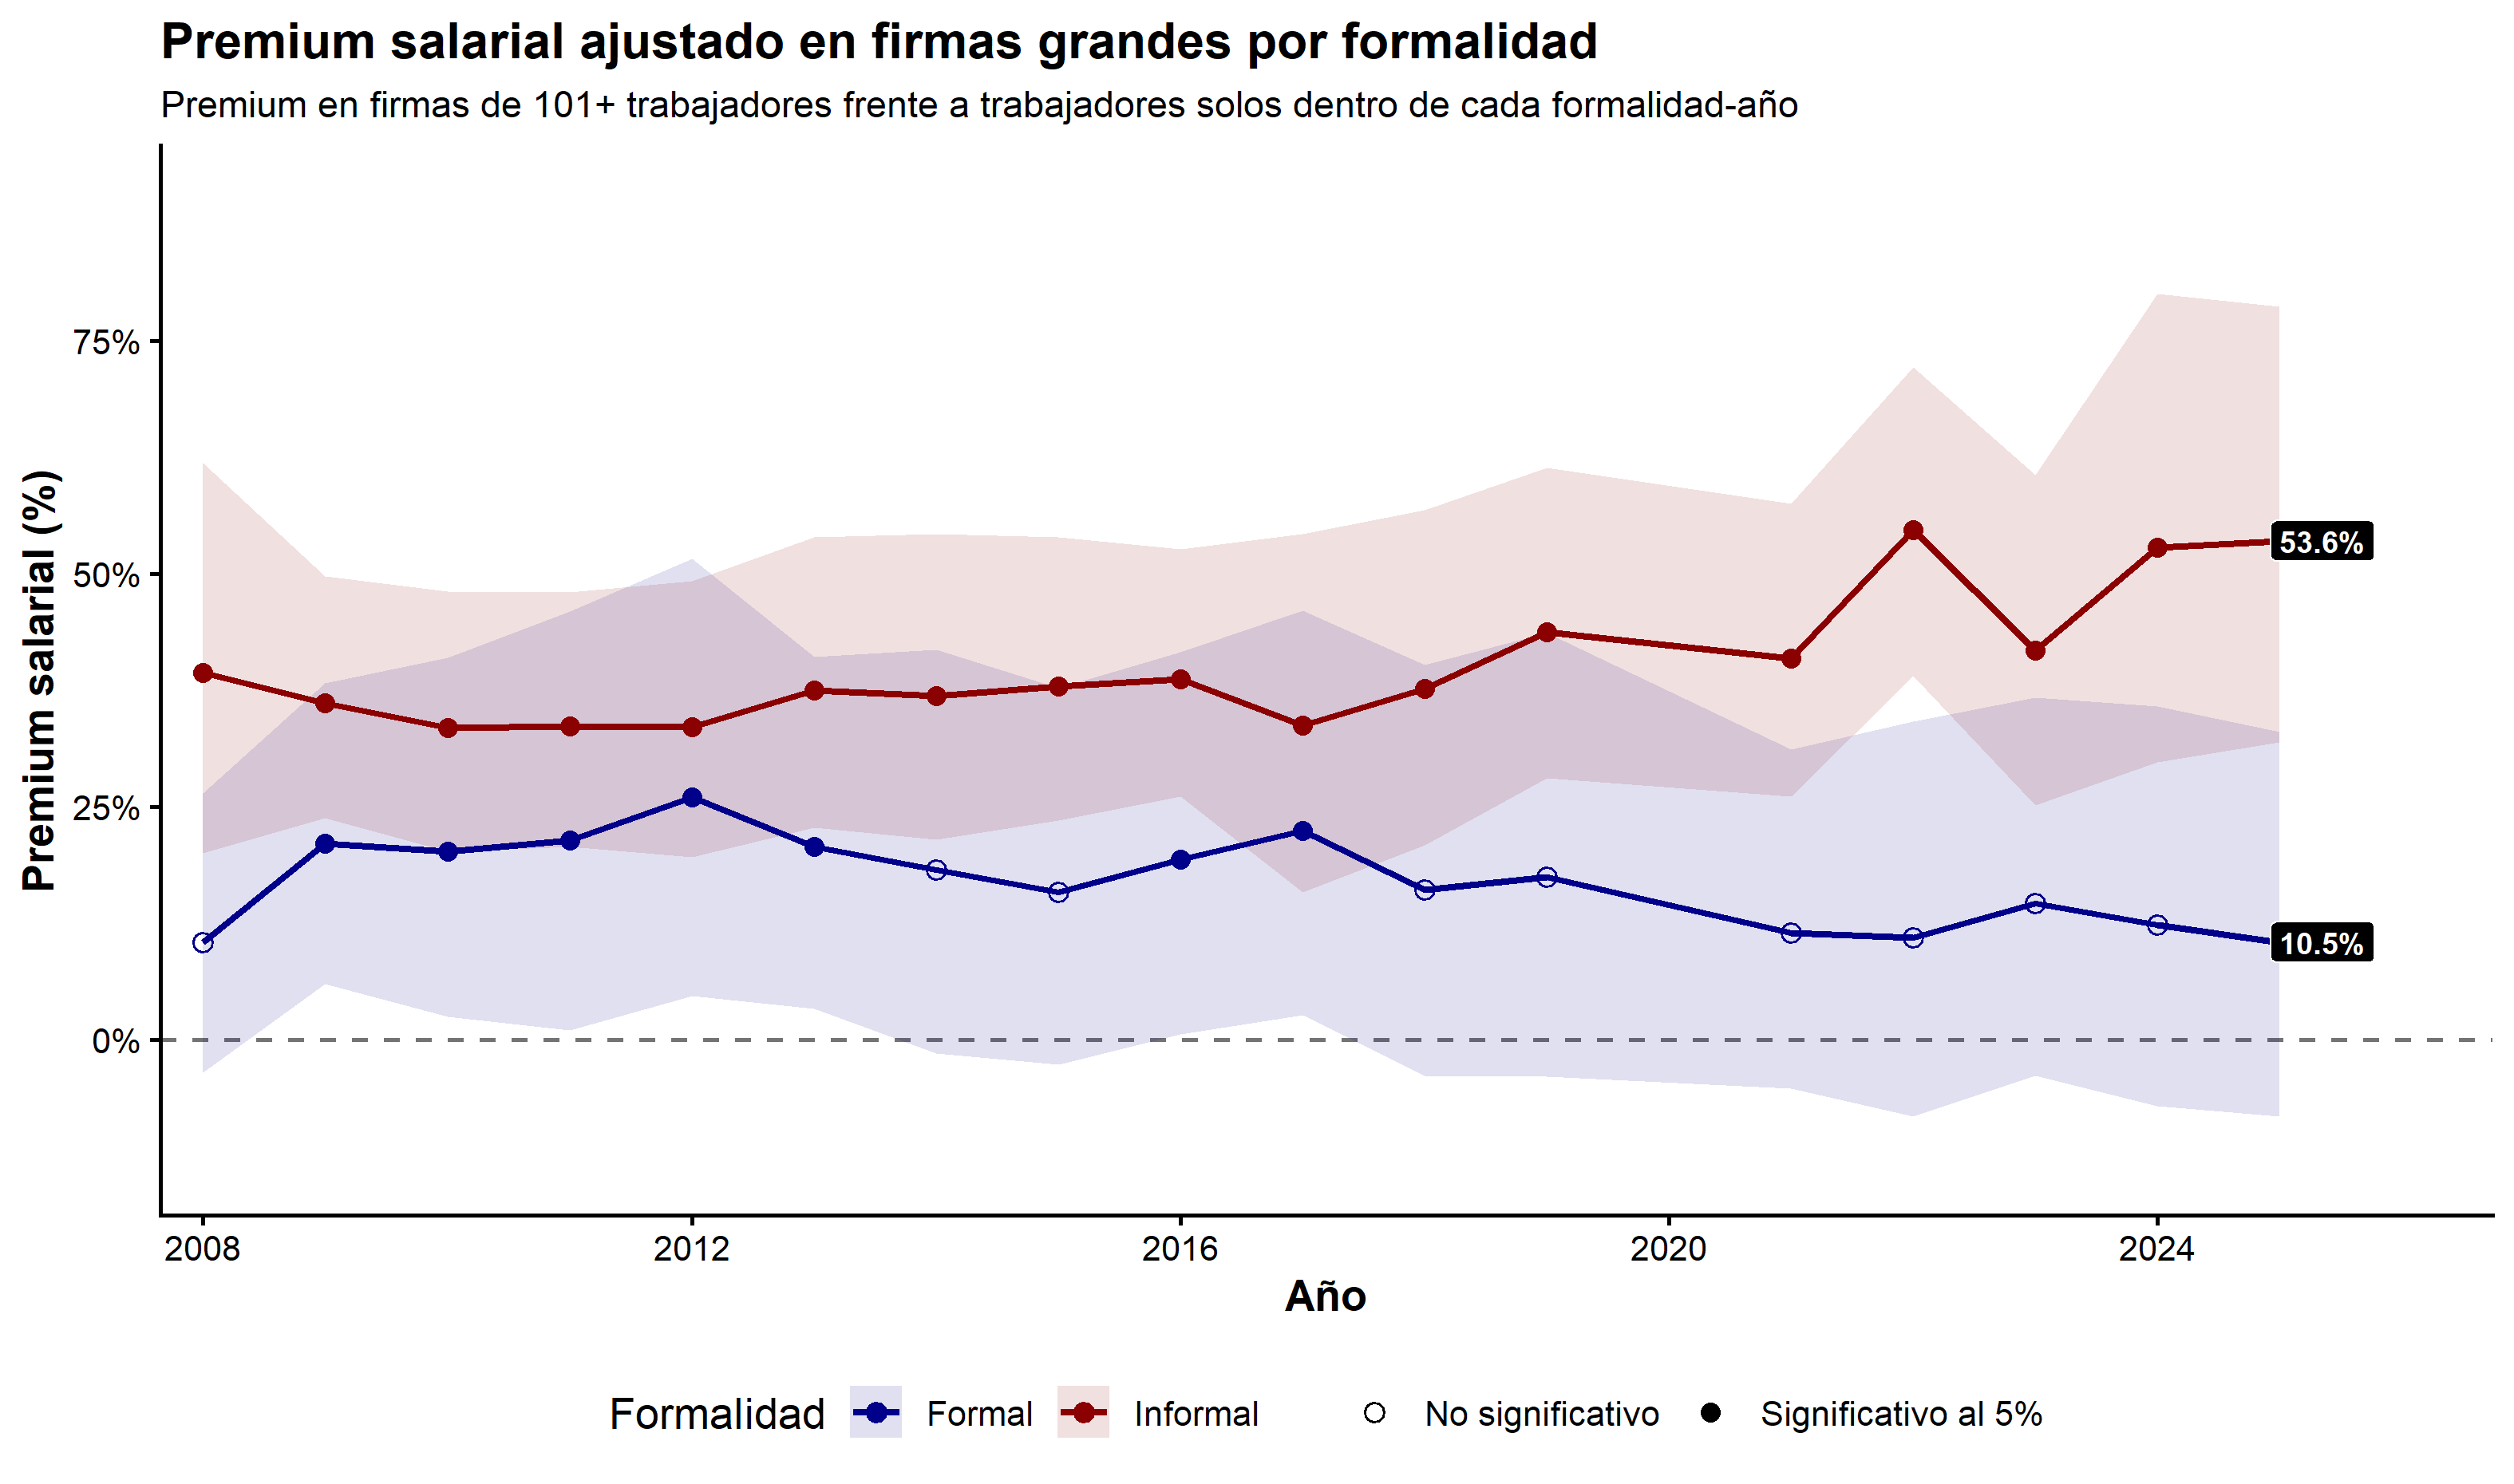
\includegraphics[width=0.95\textwidth,height=0.80\textheight,keepaspectratio]{fig75_es.png}

  \fuente{Prima de 101+ frente a solo, estimada dentro de cada grupo de formalidad. Se omite 2020.}
\end{frame}

\sectionframe{6. Elasticidad y comparación con la literatura}

\begin{frame}{Por qué estimar una elasticidad aproximada}
  \idea{El paper usa categorías de tamaño, pero la literatura suele reportar elasticidades salario-tamaño.}

  \vspace{0.35cm}
  \begin{itemize}
    \item La GEIH reporta tamaño de empresa por intervalos.
    \item Asignamos valores representativos a cada intervalo: 1, 2,5, 4,5, 8, 15, 25, 40,5, 75,5 y 150.
    \item La elasticidad es solo un ejercicio de comparación con la literatura.
    \item Las estimaciones categóricas siguen siendo el resultado principal.
  \end{itemize}
\end{frame}

\begin{frame}{Benchmark internacional}
  \idea{La elasticidad condicional colombiana es alta frente a la literatura, y esa diferencia viene principalmente del empleo informal.}

  \vspace{0.25cm}
  \begin{center}
  \small
  \begin{tabular}{lcc}
    \toprule
    Especificación & Elasticidad & Lectura \\
    \midrule
    Literatura: sin controles por heterogeneidad & 0,062 & Diegmann et al. \\
    Literatura: controles observables & 0,036 & Diegmann et al. \\
    Colombia: sin controles & 0,203 & Muy alta \\
    Colombia: muestra completa con controles & 0,071 & Alta frente al benchmark \\
    Colombia: formales con controles & 0,026 & Cerca del benchmark \\
    Colombia: informales con controles & 0,130 & Muy por encima del benchmark \\
    \bottomrule
  \end{tabular}
  \end{center}
\end{frame}

\sectionframe{7. Interpretación e implicaciones}

\begin{frame}{Qué sabemos}
  \begin{itemize}
    \item El ingreso real por hora aumenta con el tamaño de empresa.
    \item La prima se reduce mucho con controles, pero permanece positiva.
    \item No hay evidencia estadísticamente concluyente de declive secular.
    \item La prima condicional es especialmente fuerte dentro del empleo informal.
    \item La formalidad eleva el nivel salarial dentro de cada tamaño de empresa.
  \end{itemize}
\end{frame}

\begin{frame}{Qué no sabemos con estos datos}
  \idea{La GEIH no identifica firmas ni observa producto, capital o productividad marginal.}

  \vspace{0.35cm}
  \begin{itemize}
    \item No podemos separar completamente selección no observada de diferencias del lado de la firma.
    \item No podemos estimar efectos fijos de empleador.
    \item No podemos medir directamente productos marginales.
    \item Por eso hablamos de marcadores de fricciones, no de una prueba directa de misallocation.
  \end{itemize}
\end{frame}

\begin{frame}{Implicación de política}
  \idea{La conclusión no es favorecer empresas grandes por ser grandes.}

  \vspace{0.35cm}
  \begin{itemize}
    \item El objetivo relevante es reducir barreras que mantienen pequeñas, informales o desconectadas a unidades productivas con potencial.
    \item Como la formalidad eleva salarios dentro de cada tamaño, mover empleos hacia la formalidad sigue siendo una prioridad.
    \item Como la prima por tamaño es más fuerte entre informales, también importa que las unidades informales productivas puedan crecer, organizarse y conectarse a mercados.
    \item Ese apoyo debe ser una ruta hacia formalización, no un subsidio a permanecer informal.
  \end{itemize}
\end{frame}

\begin{frame}{Una mala lectura de política}
  \idea{Subsidios que preservan la pequeña escala pueden reforzar el problema que el paper documenta.}

  \vspace{0.35cm}
  \begin{itemize}
    \item No basta con apoyar pequeñas empresas si el apoyo no cambia productividad, formalización o acceso a mercados.
    \item No conviene crear umbrales regulatorios que hagan costoso crecer.
    \item Tampoco conviene incentivar que firmas formales se vuelvan informales para recibir beneficios.
    \item El foco debe estar en productividad, formalización, gestión, tecnología y conexión con clientes más grandes.
  \end{itemize}
\end{frame}

\begin{frame}{Conclusión}
  \idea{El tamaño de empresa está estrechamente asociado con la remuneración por hora en Colombia.}

  \vspace{0.35cm}
  \begin{itemize}
    \item La prima 101+ frente a trabajo solo es grande en promedios brutos y sigue siendo de 43,2\% con controles.
    \item El patrón no es solo una diferencia formal-informal.
    \item La prima más fuerte está dentro del empleo informal.
    \item El resultado central para política no es mover trabajadores mecánicamente a empresas grandes, sino entender por qué tantos trabajadores permanecen en unidades pequeñas, informales y de baja remuneración.
  \end{itemize}
\end{frame}

\begin{frame}{Para discusión}
  \begin{enumerate}
    \item ¿Cuánto de la prima condicional refleja selección no observada y cuánto refleja diferencias del lado de la firma?
    \item ¿Qué políticas ayudan a crecer a unidades informales productivas sin subsidiar la informalidad?
    \item ¿Qué datos permitirían pasar de una estadística diagnóstica a una prueba más directa de eficiencia allocativa?
    \item ¿Cómo conectar este resultado con productividad, educación, regulación y acceso a mercados?
  \end{enumerate}
\end{frame}

\begin{frame}{Referencias mencionadas}
  \scriptsize
  \begin{itemize}
    \item Abowd, Kramarz y Margolis (1999). High wage workers and high wage firms.
    \item Balkan y Tumen (2016). Firm-size wage gaps and informality in Turkey.
    \item Brown y Medoff (1989). The employer size-wage effect.
    \item Card, Heining y Kline (2013). Workplace heterogeneity and wage inequality.
    \item Diegmann, Müller y Schoefer (2026). The disappearing large-firm wage premium.
    \item El Badaoui, Strobl y Walsh (2010). Is there an informal employment wage penalty?
    \item Hsieh y Klenow (2009). Misallocation and manufacturing TFP.
    \item Reed (2019). The firm-size wage premium in developing economies.
  \end{itemize}
\end{frame}

\end{document}
